\documentclass[12pt]{article}
\usepackage{hyperref}
\usepackage{listings}
\usepackage[margin=1in]{geometry}
\usepackage{enumitem}
\usepackage{multicol}
\usepackage{array}
\usepackage{titlesec}
\usepackage{helvet}
\renewcommand{\familydefault}{\sfdefault}
\usepackage{amsmath}     % For math equations
\usepackage{amssymb}     % For advanced math symbols
\usepackage{amsfonts} % For math fonts
\usepackage{gvv}
\usepackage{esint}
\usepackage[utf8]{inputenc}
\usepackage{graphicx}
\usepackage{pgfplots}
\pgfplotsset{compat=1.18}
\titleformat{\section}{\bfseries\large}{\thesection.}{1em}{}
\setlength{\parindent}{0pt}
\setlength{\parskip}{6pt}
\usepackage{multirow}

\usepackage{fancyhdr}     % For custom headers and footers

\pagestyle{fancy}         % Use the fancy page style
\fancyhf{}                % Clear existing header/footer

% Header customization
\renewcommand{\headrulewidth}{0.4pt}          % Horizontal line at top
\fancyhead[L]{\textbf{GATE 2020}}                       % Page number on left
\fancyhead[R]{\textbf{ENGINEERING SCIENCES – XE}}  % Custom text on right
\cfoot{\thepage}

\usepackage[siunitx,RPvoltages]{circuitikz}
\usepackage{tikz}
\usepackage{float}
\usepackage{caption}

\begin{document}

\begin{center}
    {\large \textbf{GA - GENERAL APTITUDE}}
\end{center}



\begin{enumerate}

\item[] \textbf{Q1 - Q5 carry one mark each.}

\item Rajiv Gandhi Khel Ratna Award was conferred \_\_\_\_ Mary Kom, a six-time world champion in boxing, recently in a ceremony \_\_\_\_ the Rashtrapati Bhawan (the President’s official residence) in New Delhi.

\begin{enumerate}
\item with, at
\item on, in
\item on, at
\item to, at
\end{enumerate}
(GATE XE 2020)

\item Despite a string of poor performances, the chances of K. L. Rahul’s selection in the team are \_\_\_\_\_.

\begin{enumerate}
\item slim
\item bright
\item obvious
\item uncertain
\end{enumerate}
(GATE XE 2020)

\item Select the word that fits the analogy:

\textit{Cover : Uncover :: Associate : \_\_\_\_\_}

\begin{enumerate}
\item Unassociate
\item Inassociate
\item Disassociate
\item Misassociate
\end{enumerate}
(GATE XE 2020)

\item Hit by floods, the kharif (summer sown) crops in various parts of the country have been affected. Officials believe that the loss in production of the kharif crops can be recovered in the output of the rabi (winter sown) crops so that the country can achieve its food-grain production target of 291 million tons in the crop year 2019--20 (July--June). They are hopeful that good rains in July--August will help the soil retain moisture for a longer period, helping winter sown crops such as wheat and pulses during the November--February period.  

Which of the following statements can be inferred from the given passage?

\begin{enumerate}
\item Officials declared that the food-grain production target will be met due to good rains.
\item Officials want the food-grain production target to be met by the November--February period.
\item Officials feel that the food-grain production target cannot be met due to floods.
\item Officials hope that the food-grain production target will be met due to a good rabi produce.
\end{enumerate}
(GATE XE 2020)

\item The difference between the sum of the first $2n$ natural numbers and the sum of the first $n$ odd natural numbers is \_\_\_\_\_.

\begin{enumerate}
\item $n^2 - n$
\item $n^2 + n$
\item $2n^2 - n$
\item $2n^2 + n$
\end{enumerate}
(GATE XE 2020)

\item[] \textbf{Q6 - Q10 carry two marks each.}

\item Repo rate is the rate at which Reserve Bank of India (RBI) lends commercial banks, and reverse repo rate is the rate at which RBI borrows money from commercial banks.  

Which of the following statements can be inferred from the above passage?  

\begin{enumerate}
\item Decrease in repo rate will increase cost of borrowing and decrease lending by commercial banks.
\item Increase in repo rate will decrease cost of borrowing and increase lending by commercial banks.
\item Increase in repo rate will decrease cost of borrowing and decrease lending by commercial banks.
\item Decrease in repo rate will decrease cost of borrowing and increase lending by commercial banks.
\end{enumerate}
(GATE XE 2020)

\item $P, Q, R, S, T, U, V, W$ are seated around a circular table.  
\begin{enumerate}
\item[I.] $S$ is seated opposite to $W$.
\item[II.] $U$ is seated at the second place to the right of $R$.
\item[III.] $T$ is seated at the third place to the left of $R$.
\item[IV.] $V$ is a neighbour of $S$.
\end{enumerate}

Which of the following must be true?  

\begin{enumerate}
\item $P$ is a neighbour of $R$.
\item $Q$ is a neighbour of $R$.
\item $P$ is not seated opposite to $Q$.
\item $R$ is the left neighbour of $S$.
\end{enumerate}
(GATE XE 2020)

\item The distance between Delhi and Agra is $233$ km. A car $P$ started travelling from Delhi to Agra and another car $Q$ started from Agra to Delhi along the same road $1$ hour after the car $P$ started. The two cars crossed each other $75$ minutes after the car $Q$ started. Both cars were travelling at constant speed. The speed of car $P$ was $10$ km/hr more than the speed of car $Q$. How many kilometers the car $Q$ had travelled when the cars crossed each other?  

\begin{enumerate}
\item 66.6
\item 75.2
\item 88.2
\item 116.5
\end{enumerate}
(GATE XE 2020)

\item For a matrix $M = [m_{ij}],\ i,j=1,2,3,4$, the diagonal elements are all zero and $m_{ij} = -m_{ji}$.  
The minimum number of elements required to fully specify the matrix is \_\_\_\_.  

\begin{enumerate}
\item 0
\item 6
\item 12
\item 16
\end{enumerate}
(GATE XE 2020)

\item The profit shares of two companies P and Q are shown in the figure. If the two companies have invested a fixed and equal amount every year, then the ratio of the total revenue of company P to the total revenue of company Q, during 2013--2018 is \_\_\_\_.  

\begin{figure}[H]
    \centering
    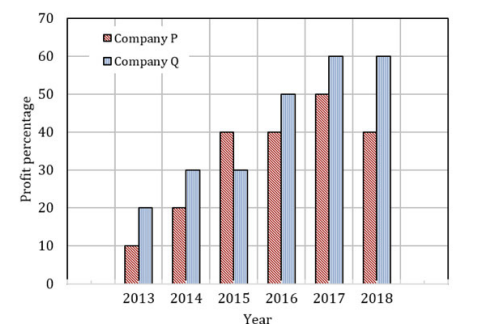
\includegraphics[width=0.5\columnwidth]{figs/ass4_0_q10.png}
    \caption{}
    \label{fig:placeholder}
\end{figure}

\begin{enumerate}
\item 15:17
\item 16:17
\item 17:15
\item 17:16
\end{enumerate}
(GATE XE 2020)


\end{enumerate}

\newpage

\begin{center}
    {\Large \textbf{A : Engineering Mathematics (compulsory)}}
\end{center}  

  

\begin{enumerate}

\item[] \textbf{Q1 - Q7 carry one mark each.} 

\item Let $A$ be a $4 \times 3$ non-zero matrix and let $b$ be a $4 \times 1$ column vector. Then $Ax = b$ has  
\begin{enumerate}
\item a solution for every $b$.  
\item no solution for some $b$.  
\item a solution only when $b = 0$.  
\item a solution if $b$ and the columns of $A$ form a linearly independent set.  
\end{enumerate}
(GATE XE 2020)

\item Let $x_0, x_1, x_2, \ldots$ be the sequence generated by the Newton-Raphson method applied to the function $f(x) = x^2 - 2x + 2$ with $x_0 = 1$. Then the sequence  
\begin{enumerate}
\item converges to $0$.  
\item becomes unbounded.  
\item converges to a root of $f(x)$.  
\item does not converge.  
\end{enumerate}
(GATE XE 2020)

\item Let $z(t)$ be the solution of the initial value problem  
$$
\frac{d^2 z}{dt^2} = bz,\quad z(0) = 0,\quad \frac{dz}{dt}(0) = 1 \quad \text{for } t \geq 0.
$$
If the planar curve parameterized by $t$ having $x$--coordinate $z(t)$ and $y$--coordinate $\frac{dz}{dt}$ is closed, then necessarily  
\begin{enumerate}
\item $b > 0$.  
\item $b < 0$.  
\item $b \leq 0$.  
\item $b$ is a non-zero rational number.  
\end{enumerate}
(GATE XE 2020)

\item Let $z$ be a complex number. Then the series $\sum_{n=0}^{\infty} \frac{z^n}{(2n)!}$ 
  \begin{enumerate}
    \item converges for all $z$.
    \item converges for $|z|\leq 1$ and diverges for $|z|>1$.
    \item converges for $z=0$ and diverges for any $z \neq 0$.
    \item converges for $|z|<1$ and diverges for $|z|\geq 1$.
  \end{enumerate}
(GATE XE 2020)

\item Let $\vec{F}(x,y,z)=ax\hat{i}-(bz\hat{j}+cy)\hat{k}$ be a vector field whose curl is zero. Then necessarily
  \begin{enumerate}
    \item $a=b=c$
    \item $a=-b=c$
    \item $b=c$
    \item $b=-c$
  \end{enumerate}
  (GATE XE 2020)

\item Let $f(x)$ be a continuous function on the real line such that for any $x$, 
  $$\int_{0}^{x} f(t) \, dt = x^2 (1+x^2).$$
  Then $f(2)$ is \_\_\_\_\_

  (GATE XE 2020)

\item The number of points at which the function $f(x,y) = \frac{x^2}{2} + \frac{y^4}{4} - \frac{y^2}{2}$ has local minima is \_\_\_\_\_

  (GATE XE 2020)


\item[] \textbf {Q8 -- Q11 carry two marks each.}



\item Let $f(t)$ be a real-valued differentiable function on $(-1,1)$ such that $f(0)=0$ and $\left| \frac{df}{dt} \right| < 1$ for $0 < t < 1$. Then the series $\sum f(0.5^n)$
  \begin{enumerate}
    \item converges but not absolutely.
    \item is unbounded.
    \item converges absolutely.
    \item is bounded but does not converge.
  \end{enumerate}
  (GATE XE 2020)

\item Let $X$ be a random variable with probability density function
  $$
  f(x) = \begin{cases}
  exp(-t),&  \text{for } t\geq0 \\
  0, & \text{for } t< 0
  \end{cases}
  $$
  where $0 < a < b$. Then the probability $P(X \leq b \, | \, X \geq a)$ depends only on
  \begin{enumerate}
    \item $b-a$
    \item $b$
    \item $a$
    \item $a+b$
  \end{enumerate}
  (GATE XE 2020)

  \item Let $A$ be a $3 \times 3$ matrix such that $A^2 = 4I$. Then it is necessary that
  \begin{enumerate}
    \item $A$ is the identity matrix or the zero matrix.
    \item The determinant of $A$ is either $0$ or $1$.
    \item The rank of $A$ is $3$.
    \item $A$ has one imaginary eigenvalue.
  \end{enumerate}
  (GATE XE 2020)

  \item Players $A$ and $B$ take turns to throw a fair dice with six faces. If $A$ is the first player to throw, then the probability of $B$ being the first one to get a six is \_\_\_\_\_ (round off to two decimal places).
  
  (GATE XE 2020)


\end{enumerate}

\begin{center}
    \textbf{END OF SECTION - A}
\end{center}

\newpage
\begin{center}
    {\Large \textbf{B : FLUID MECHANICS} }
\end{center}

\begin{enumerate}

\item[] \textbf{Q1 - Q9 carry one mark each.}

\item Figures given below show the velocity and shear stress profiles for the flow in a duct. 
In each option, `1' represents velocity profile and `2' represents shear stress profile.

Choose the correct option that closely represents the turbulent flow condition.  

\begin{enumerate}
\item \begin{figure}[H]
    \centering
    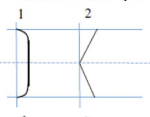
\includegraphics[width=0.5\columnwidth]{figs/ass4_b_q1_a.png}
    \caption{}
    \label{fig:placeholder}
\end{figure} 
\item \begin{figure}[H]
    \centering
    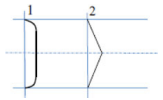
\includegraphics[width=0.5\columnwidth]{figs/ass4_b_q1_b.png}
    \caption{}
    \label{fig:placeholder}
\end{figure}
\item \begin{figure}[H]
    \centering
    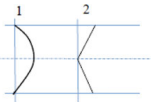
\includegraphics[width=0.5\columnwidth]{figs/ass4_b_q1_c.png}
    \caption{}
    \label{fig:placeholder}
\end{figure} 
\item \begin{figure}[H]
    \centering
    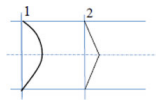
\includegraphics[width=0.5\columnwidth]{figs/ass4_b_q1_d.png}
    \caption{}
    \label{fig:placeholder}
\end{figure} 
\end{enumerate}
(GATE XE 2020)

\item The variation of shear stress $\tau$ against strain rate $\dfrac{du}{dy}$ is given in the figure. 
Identify the line/curve among P, Q, R and S, that represents an ideal fluid. 

\begin{figure}[H]
    \centering
    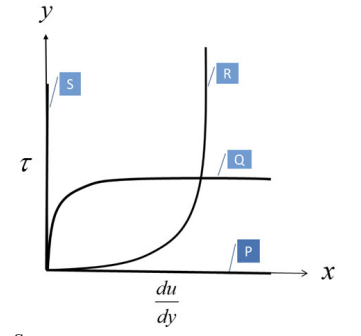
\includegraphics[width=0.5\columnwidth]{figs/ass4_b_q2.png}
    \caption{}
    \label{fig:placeholder}
\end{figure}

\begin{enumerate}
\item S  
\item P  
\item Q  
\item R  
\end{enumerate}
(GATE XE 2020)

\item A body is under stable equilibrium in a homogeneous fluid, where CG and CB are center of gravity and center of buoyancy, respectively.  

Two statements `P' and `Q' are given below:  

P: For a fully submerged condition, CG should always be below CB. \\  
Q: For a floating body, CG need not be below CB. \\  

Choose the option that is valid for the present situation.  

\begin{enumerate}
\item P is False; Q is True when metacentre is below CG  
\item P is False; Q is True when metacentre is above CG  
\item P is True; Q is True when metacentre is below CG  
\item P is True; Q is True when metacentre is above CG  
\end{enumerate}
(GATE XE 2020)

\item A laminar hydrodynamic boundary layer over a smooth flat plate is shown in the figure. The shear stress at the wall is denoted by $\tau_w$. Which one of the following conditions is correct.  

\begin{figure}[H]
    \centering
    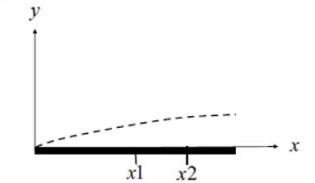
\includegraphics[width=0.5\columnwidth]{figs/ass4_b_q4.png}
    \caption{}
    \label{fig:placeholder}
\end{figure}

\begin{enumerate}
\item Pressure is varying along $x$ and $(\tau_w)_{x1} > (\tau_w)_{x2}$  
\item Pressure is constant along $x$ and $(\tau_w)_{x2} > (\tau_w)_{x1}$  
\item Pressure is constant along $x$ and $(\tau_w)_{x1} > (\tau_w)_{x2}$  
\item Pressure is varying along $x$ and $(\tau_w)_{x2} > (\tau_w)_{x1}$  
\end{enumerate}
(GATE XE 2020)

\item A non-dimensional number known as \textbf{Weber number} is used to characterize which one of the following flows.  


\begin{enumerate}
\item Motion of fluid in open channel  
\item Motion of fluid droplets  
\item Motion of fluid at high velocity  
\item Motion of fluid through a pipe  
\end{enumerate}
(GATE XE 2020)

\item A uniform approach flow is subjected to an unsteady and periodic flapping plate as shown in the Figure. Tracer is released to obtain flow visualization lines, which are marked as ‘P’, ‘Q’ and ‘R’.  

\begin{figure}[H]
    \centering
    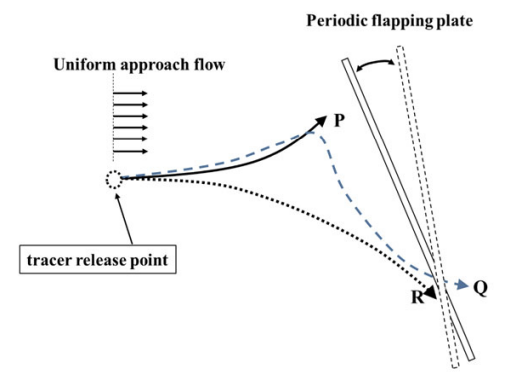
\includegraphics[width=0.5\columnwidth]{figs/ass4_b_q6.png}
    \caption{}
    \label{fig:placeholder}
\end{figure}

Choose the correct option that the line ‘R’ represents  
\begin{enumerate}
\item Streakline
\item Streamline
\item Pathline
\item Timeline
\end{enumerate}
(GATE XE 2020)

\item The volume flow between any two points not lying on the same streamline in a flow field is equal to  
\begin{enumerate}
\item Change in strain rate between the points
\item Change in vorticity between the points
\item Change in potential function between the points
\item Change in stream function between the points
\end{enumerate}
(GATE XE 2020)

\item A liquid flow through a horizontal smooth pipe of diameter $5 \ \text{cm}$ and discharges into a collection tank of dimension $50 \ \text{cm} \times 50 \ \text{cm} \times 50 \ \text{cm}$. Time taken for a $10 \ \text{cm}$ rise of liquid level in the collection tank is $40 \ \text{s}$.  

The flow velocity in the pipe is \_\_\_\_\_\_ m/s (rounded off to two decimal places).

(GATE XE 2020)

\item The potential function for a two dimensional incompressible flow field is given as:  
$
\phi = \frac{x^3}{3} - x y^2
$

Magnitude of the velocity vector at point $(2,1)$ is \_\_\_\_\_\_ m/s  

(GATE XE 2020)

\item Column I represents a list of elementary plane flows and Column II represents flow past geometry obtained by superposition of these elementary plane flows.

\begin{table}[H]
\centering
\begin{tabular}{l l}

Column I &  Column II  \\

P: Source, Sink, Uniform flow  & 1: Rankine half body  \\
Q: Doublet, Uniform flow & 2: Rotating Cylinder  \\
R: Source, Uniform flow & 3: Rankine oval  \\
S: Doublet, Free vortex, Uniform flow  & 4: Cylinder  \\
\end{tabular}
\caption{}
\label{}
\end{table}

The correct match between Columns I and II is

\begin{enumerate}
\item P-3; Q-2; R-1; S-4
\item P-1; Q-2; R-3; S-4
\item P-3; Q-4; R-1; S-2
\item P-1; Q-4; R-3; S-2
\end{enumerate}
(GATE XE 2020)

\item The velocity field for a flow is $\vec{V} = 5\hat{i} + 2xt\hat{j} + 2ty\hat{k}$, where $t$ is time. Choose the correct option representing the total acceleration at $(x,y,z,t)$.

\begin{enumerate}
\item $5\hat{i} + 2(x+z)\hat{j} + 2(t+y)\hat{k}$
\item $5\hat{i} + t(10z+4xy)\hat{j} + (2y+4xzt)\hat{k}$
\item $5\hat{i} + 2y\hat{k}$
\item $2t(2xy+5z)\hat{j} + 4xzt \hat{k}$
\end{enumerate}
(GATE XE 2020)

\item An incompressible viscous fluid is placed between two infinite horizontal parallel plates as shown in Figure. The plates move in opposite direction with constant velocities $U_1$ and $U_2$. The pressure gradient in the x-direction is zero and the only body force is due to the fluid weight. The flow is steady, laminar and two-dimensional. Assume velocity component in y direction to be zero.

\begin{figure}[H]
    \centering
    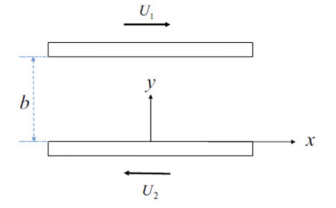
\includegraphics[width=0.5\columnwidth]{figs/ass4_b_q12.png}
    \caption{}
    \label{fig:placeholder}
\end{figure}

The correct expression for the velocity distribution between the plates is:

\begin{enumerate}
\item $\left (\frac{U_1 + U_2}{b}\right) y - U_2$
\item $\left (\frac{U_1 - U_2}{b}\right) y - U_1$
\item $\left (\frac{U_1 + U_2}{b}\right) y + U_2$
\item $\left (\frac{U_1 + U_2}{b}\right) y + U_1$
\end{enumerate}
(GATE XE 2020)

\item The stream function of a flow field is $\Psi = k(x^2 - y^2 x)$ where $k$ is a constant.  
Which one of the following represents the vorticity?

\begin{enumerate}
\item $-2k$
\item $2k(x+1)$
\item $2k(x-1)$
\item $-2k(x+1)$
\end{enumerate}
(GATE XE 2020)

\item Consider a two dimensional, incompressible steady flow of a Newtonian fluid in which the velocity field is $u = -2xy, \ v = y^2 - x^2$.  
Pressure gradients in the $x$- and $y$-directions are

\begin{enumerate}
\item $\dfrac{\partial p}{\partial x} = -2\rho(xy^2 + x^3),
       \dfrac{\partial p}{\partial y} = -2\rho(x^2 y + y^3)$
\item $\dfrac{\partial p}{\partial x} = -2\rho(xy^2 - x^3),
       \dfrac{\partial p}{\partial y} = -2\rho(x^2 y + y^3)$
\item $\dfrac{\partial p}{\partial x} = -2\rho(xy^2 + x^3),  
       \dfrac{\partial p}{\partial y} = -2\rho(x^2y - y^3)$
\item $\dfrac{\partial p}{\partial x} = -2\rho(xy^2 - x^3), 
       \dfrac{\partial p}{\partial y} = -2\rho(x^2y - y^3)$
\end{enumerate}
(GATE XE 2020)

\item A hydroelectric power plant takes in $30 \ \text{m}^3/\text{s}$ of water through its turbine and discharges it to the atmosphere with $V_2 = 2 \ \text{m/s}$.  
The total head loss in the turbine and penstock system is $20 \ \text{m}$.  
(Assume turbulent flow with kinetic energy correction factor as $1.1$.  
Density of water is $1000 \ \text{kg/m}^3$ and acceleration due to gravity, $g = 10 \ \text{m/s}^2$).  

The net head available to the turbine for power generation is \_\_\_\_\_ m.  
(Rounded off to one decimal place).

\begin{figure}[H]
    \centering
    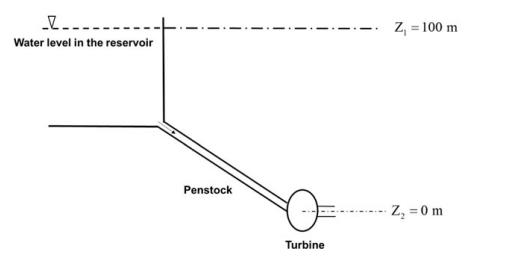
\includegraphics[width=0.5\columnwidth]{figs/ass4_b_q15.png}
    \caption{}
    \label{fig:placeholder}
\end{figure}
(GATE XE 2020)

\item Water flows at an average velocity, $v$ of $10 \, \text{m/s}$ through a horizontal smooth tube of diameter, $d = 5 \, \text{cm}$. The friction factor, $f$ is $0.02$. Head loss is obtained using Darcy-Weisbach relation $\dfrac{flv^2}{2gd}$. The fluid pressure, $p$ measured at various stations are reported in the table below. The length of the pipe, $l$ between station 0 and station 6 is $6 \, \text{m}$.

\begin{table}
\centering \caption{} \label{}
\begin{tabular}{|c|c|c|c|c|c|c|c|}
\hline
\text{Station} & 0 & 1 & 2 & 3 & 4 & 5 & 6 \\
\hline
p, \, \text{kPa} & 304 & 273 & 255 & 240 & 226 & 213 & - \\
\hline
\end{tabular}
\end{table}


If acceleration due to gravity, $g = 10 \, \text{m/s}^2$ and density of water $= 1000 \, \text{kg/m}^3$, then the fluid pressure at station 6 is \_\_\_\_\_\_ kPa.  
(Rounded off to one decimal place)

(GATE XE 2020)

\item A sphere model of $10 \, \text{cm}$ diameter is tested in water flowing at $2 \, \text{m/s}$. The drag force is measured as $5 \, \text{N}$. Prototype of $1.5 \, \text{m}$ in diameter is tested in air with dynamic similarity conditions. (Density of water is $1000 \, \text{kg/m}^3$, density of air is $1.2 \, \text{kg/m}^3$, viscosity of water is $0.001 \, \text{Ns/m}^2$ and viscosity of air is $1.78 \times 10^{-5} \, \text{Ns/m}^2$).  

Drag force experienced by the prototype is \_\_\_\_\_\_ N (rounded off to two decimal places).

(GATE XE 2020)

\item A liquid of viscosity $1.74 \times 10^{-3} \, \text{Ns/m}^2$ is flowing through a horizontal capillary tube of diameter $0.5 \, \text{mm}$. The flow in the tube is steady, incompressible, and fully developed laminar flow. The pressure drop across two locations spaced $1 \, \text{m}$ apart in the tube is $1.0 \, \text{MPa}$.  

The flow rate in the tube is \_\_\_\_\_\_ mm$^3$/s.

(GATE XE 2020)

\item A venturimeter with $75 \, \text{mm}$ diameter throat is placed in a $150 \, \text{mm}$ diameter pipeline carrying water at $25^\circ \text{C}$. The pressure drop between the upstream tap and the venturi throat is $40 \, \text{kPa}$. (Density of water $= 1000 \, \text{kg/m}^3$).  

The flow rate is \_\_\_\_\_\_\_ m$^3$/s (rounded off to three decimal places).

(GATE XE 2020)

\item A water jet with velocity $\bar{V}_{jet}$ impinges normal to a moving flat plate with velocity $\bar{V}_{plate}$ such that the jet splits equally into two halves as shown in Figure.  

The jet cross-sectional area is $2 \,\text{cm}^2$, $\bar{V}_{jet}$ is $20 \,\text{m/s}$ and $\bar{V}_{plate}$ is $10 \,\text{m/s}$ and density of water is $1000 \,\text{kg/m}^3$. Consider steady flow and neglect weight of the jet, weight of the plate and frictional losses.  

The absolute value of the force required to keep the plate moving at constant velocity $\bar{V}_{plate}$ is \_\_\_\_\_\_\_ N.  

\begin{figure}[H]
    \centering
    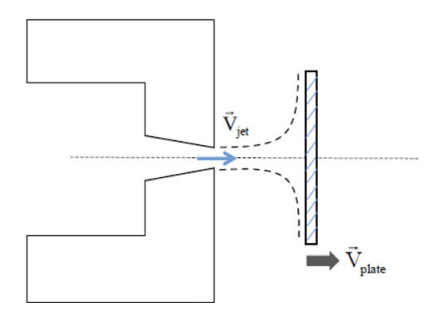
\includegraphics[width=0.5\columnwidth]{figs/ass4_b_q20.png}
    \caption{}
    \label{fig:placeholder}
\end{figure}

(GATE XE 2020)

\item In an inverted manometer (as shown in the Figure), the pressure difference, 
$P_{B} - P_{A}$, is $100 \,\text{kPa}$.  

Use specific gravity of oil as $0.8$, density of water as $1000 \,\text{kg/m}^3$, density of mercury as $13600 \,\text{kg/m}^3$ and acceleration due to gravity as $10 \,\text{m/s}^2$.  

The height of the water column, $H$, is \_\_\_\_\_\_ cm. (rounded off to one decimal place)  

\begin{figure}[H]
    \centering
    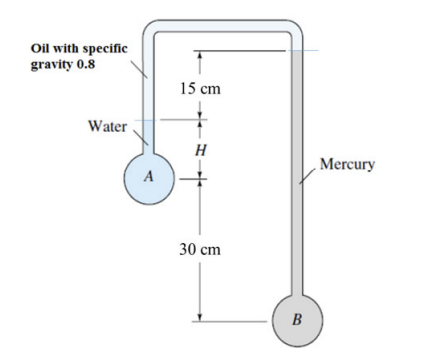
\includegraphics[width=0.5\columnwidth]{figs/ass4_b_q21.png}
    \caption{}
    \label{fig:placeholder}
\end{figure}

(GATE XE 2020)  

\item An incompressible, steady flow with uniform velocity condition at the inlet between parallel plates is shown in Figure. The flow develops into a parabolic laminar profile with  
$
u = \alpha y (y_{0} - y)
$
at the downstream end, where $\alpha$ is a constant. Assume unit depth of the plate.  
For $U_{0} = 7.5 \,\text{cm/s}$, $y_{0} = 3 \,\text{cm}$ and the fluid with density $\rho = 800 \,\text{kg/m}^3$,  

the value of $\alpha$ is \_\_\_\_\_\_\_.  

\begin{figure}[H]
    \centering
    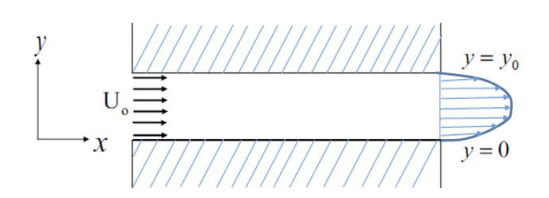
\includegraphics[width=0.5\columnwidth]{figs/ass4_b_q22.png}
    \caption{}
    \label{fig:placeholder}
\end{figure}

(GATE XE 2020)

\end{enumerate}

\begin{center}
    \textbf{END OF SECTION - B}
\end{center}

\newpage
\begin{center}
    {\Large \textbf{C :MATERIALS SCIENCE} }
\end{center}

\begin{enumerate}

\item[] \textbf{Q1 - Q9 carry one mark each.}

\item A Pb-Sn sample of eutectic composition, containing $\alpha$- and $\beta$- phases, is examined in a scanning electron microscope. The $\alpha$-phase contains $\sim 97$ wt\% Pb (atomic number 82) while $\beta$-phase contains $\sim 99$ wt\% Sn (atomic number 50). The ratio of number of backscattered electrons escaping from $\alpha$-phase to that from $\beta$-phase would be:
\begin{enumerate}
    \item Less than 1
    \item Equal to 1
    \item Greater than 1
    \item Equal to 0
\end{enumerate}
(GATE XE 2020)

\item Smallest or minimum feature size that can be theoretically resolved in an optical microscope does NOT depend on:
\begin{enumerate}
    \item Refractive index of the medium between the lens and the focal point
    \item Intensity of radiation
    \item Wavelength of radiation
    \item Numerical aperture of the objective lens
\end{enumerate}
(GATE XE 2020)

\item Following diagram shows a square 2-D lattice with a hexagonal motif (dark colored). The rotational symmetry element that must be present in the system is:

\begin{figure}[H]
    \centering
    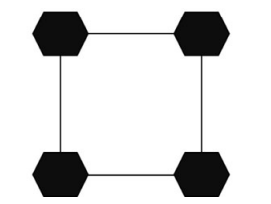
\includegraphics[width=0.5\columnwidth]{figs/ass4_c_q3.png}
    \caption{}
    \label{fig:placeholder}
\end{figure}
\begin{enumerate}
    \item Six-fold rotation
    \item Two-fold rotation
    \item Three-fold rotation
    \item Four-fold rotation
\end{enumerate}
(GATE XE 2020)

\item Density of states, $D(E)$, in a three dimensional solid varies with energy $(E)$ as
\begin{enumerate}
    \item $E^{1/2}$
    \item $E^0$
    \item $E^{-1/2}$
    \item $E^{3/2}$
\end{enumerate}
(GATE XE 2020)

\item The variation of molar volume ($V_m$) of a liquid showing glass transition temperature ($T_g$) while cooling from its melting temperature ($T_m$) is depicted by: 

\begin{figure}[H]
    \centering
    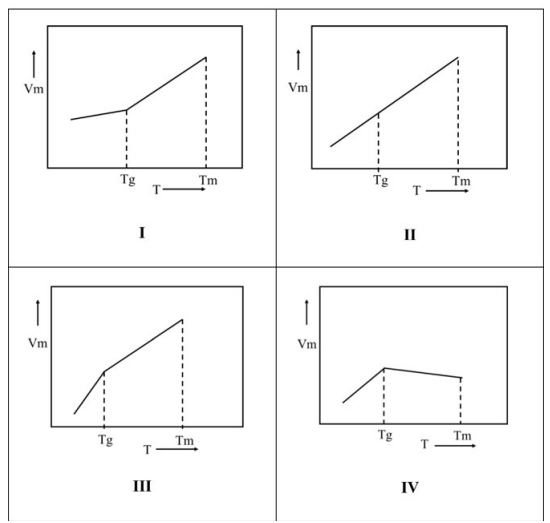
\includegraphics[width=0.8\columnwidth]{figs/ass4_c_q5.png}
    \caption{}
    \label{fig:placeholder}
\end{figure}

\begin{enumerate}
\item I  
\item II  
\item III  
\item IV  
\end{enumerate}

(GATE XE 2020)

\item Find the correct match between polymer name in Column I and the monomer type in Column II.  

\begin{figure}[H]
    \centering
    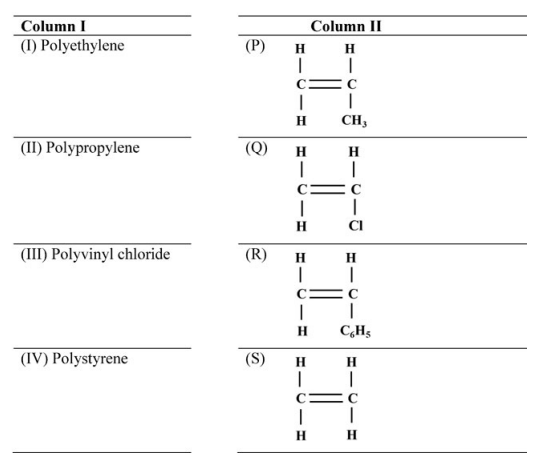
\includegraphics[width=0.8\columnwidth]{figs/ass4_c_q6.png}
    \caption{}
    \label{fig:placeholder}
\end{figure}


\begin{enumerate}
\item I-P, II-S, III-R, IV-Q
\item I-R, II-Q, III-S, IV-P
\item I-S, II-P, III-Q, IV-R
\item I-S, II-R, III-Q, IV-P
\end{enumerate}

(GATE XE 2020)

\item A ceramic has a fracture toughness ($K_{IC}$) of $1 \,\text{MPa}\,\text{m}^{1/2}$.  
If this ceramic is to be exposed to a maximum stress ($\sigma$) of $200 \,\text{MPa}$,  
the maximum value of half crack length $a$ (in micrometer, $\mu$m), below which the material does not fail, is $\_\_\_\_\_$ $\mu$m  
(\textit{round off to one decimal place}).  
Loading condition for the sample is shown in the schematic.  
Assume geometrical factor $Y = 1.2$.  

\begin{figure}[H]
    \centering
    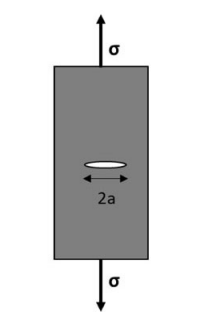
\includegraphics[width=0.5\columnwidth]{figs/ass4_c_q7.png}
    \caption{}
    \label{fig:placeholder}
\end{figure}


(GATE XE 2020)

\item A ceramic material is periodically heated and cooled between $25^\circ$C and a higher temperature, $T_f$. During thermal cycling, the material remains dimensionally constrained. The material can withstand a maximum compressive stress of $200$ MPa without failure. Material’s coefficient of thermal expansion is $7.5 \times 10^{-6}$ $^\circ$C$^{-1}$ and modulus of elasticity $(E)$ is $200$ GPa. The lowest value of $T_f$ (in $^\circ$C) at which material will fail is \underline{\hspace{1cm}} $^\circ$C (round-off to the nearest integer). Assume that there is no plastic deformation during thermal cycling.  

(GATE XE 2020)

\item During homogeneous solidification of a liquid metal, the radius of critical nucleus (in nanometer, nm) at a temperature $T_s$ which is below the melting point $(T_m)$ is \underline{\hspace{1cm}} nm (round-off to one decimal place). Given that $\gamma_{sl}$ (solid liquid interfacial energy) is $0.18$ J.m$^{-2}$ and $\Delta G_v$ (change in volume free energy upon transformation from liquid to solid) at $T_s$ is $0.18 \times 10^9$ J.m$^{-3}$.  

(GATE XE 2020)

\item[] \textbf{Q10 - Q22 carry two marks each.}

\item Read the two statements related to sintering and select the correct option.  

Statement-1: Sintering in vacuum leads to improved densification as compared to sintering under ambient (at atmospheric pressure) condition.  

Statement-2: Closed pores formed during sintering inhibit full densification.  

\begin{enumerate}
\item Both Statement-1 and Statement-2 are FALSE  
\item Both Statement-1 and Statement-2 are TRUE  
\item Statement-1 is TRUE but Statement-2 is FALSE  
\item Statement-1 is FALSE but Statement-2 is TRUE  
\end{enumerate}

(GATE XE 2020)

\item Select the correct option that appropriately matches the process to the material/product that can be fabricated using them.  

\begin{table}[H]
\centering
\caption{} \label{}
\begin{tabular}{|l|l|}
\hline
\textbf{Process} & \textbf{Material/Product} \\ \hline
(I) Powder processing      & (P) Organic semiconductor thin films \\ \hline
(II) Spin coating          & (Q) Single crystal silicon \\ \hline
(III) Czochralski process  & (R) Poly-silicon \\ \hline
(IV) Chemical vapor deposition & (S) Porous bronze bearings \\ \hline
\end{tabular}
\end{table}

\begin{enumerate}
\item I-S, II-P, III-R, IV-Q  
\item I-S, II-R, III-Q, IV-P  
\item I-S, II-P, III-Q, IV-R  
\item I-P, II-R, III-Q, IV-S  
\end{enumerate}

(GATE XE 2020)

\item Consider a FCC structured metal with lattice parameter $a = 3.5$ \AA. If the material is irradiated using X-rays of wavelength $\lambda = 1.54056$ \AA, the Bragg angle ($2\theta$) corresponding to the fourth reflection will be:  

\begin{enumerate}
    \item $88.21^\circ$
    \item $76.99^\circ$
    \item $99.35^\circ$
    \item $93.80^\circ$
\end{enumerate}

(GATE XE 2020)

\item The number of Schottky defects per mole of KCl at $300^{\circ} \mathrm{C}$ under equilibrium condition will be:

Given:  

Activation energy for the formation of Schottky defect $= 250 \,\text{kJ.mol}^{-1}$  
Avogadro number $= 6.023 \times 10^{23}\,\text{mol}^{-1}$  
Universal Gas Constant $= 8.314 \,\text{J.K}^{-1}\text{.mol}^{-1}$  

\begin{enumerate}
\item $1.21 \times 10^{18}$
\item $1.52 \times 10^{16}$
\item $9.75$
\item $2.42 \times 10^{12}$
\end{enumerate}

(GATE XE 2020)

\item In an industry, the probability of an accident occurring in a given month is $\tfrac{1}{100}$.  
Let $P(n)$ denote the probability that there will be no accident over a period of $n$ months. Assume that the events of individual months are independent of each other.  

The smallest integer value of $n$ such that $P(n) \leq \tfrac{1}{2}$ is \_\_\_\_\_ (round off to the nearest integer).

(GATE XE 2020)

\item For a FCC metal, the ratio of surface energy of $\{111\}$ surface to $\{100\}$ surface is \_\_\_\_\_ (round-off to two decimal places). Assume that only the nearest neighbor broken bonds contribute to the surface energy.

(GATE XE 2020)

\item Pure silicon (Si) has a band gap ($E_g$) of $1.1 \,\text{eV}$. This Si is doped with $1$ ppm (parts per million) of phosphorus atoms. Si contains $5 \times 10^{28}$ atoms per m$^3$ in pure form.  

At temperature $T = 300 \,\text{K}$, the shift in Fermi energy upon doping with respect to intrinsic Fermi level of pure Si will be \_\_\_\_\_ eV (with appropriate sign and round-off to two decimal places).  

Intrinsic carrier concentration of Si, $n_i$, is given as:  
$$
n_i = 2 \left(\frac{2 \pi m k_B T}{h^2}\right)^{3/2} \exp\left(\frac{-E_g}{2 k_B T}\right)
$$

Given:  

Mass of an electron, $m = 9.1 \times 10^{-31}\,\text{kg}$  
Charge of an electron, $e = 1.6 \times 10^{-19}\,\text{C}$  
Boltzmann constant, $k_B = 1.38 \times 10^{-23}\,\text{J.K}^{-1}$  
Planck’s constant, $h = 6.6 \times 10^{-34}\,\text{J.s}$  

(GATE XE 2020)

\item The schematic diagram shows the light of intensity $I_0$ incident on a material (shaded grey) of thickness, $x$, which has an absorption coefficient, $\alpha$ and reflectance, $R$. The intensity of transmitted light is $I$. The reflection of light (of a particular wavelength) occurs at both the surfaces (surfaces indicated in the diagram). The transmittance is estimated to be \_\_\_\_\_ (round-off to three decimal places).  

Given that for the wavelength used, $\alpha = 10^3 \,\text{m}^{-1}$ and $R = 0.05$. 

\begin{figure}[H]
    \centering
    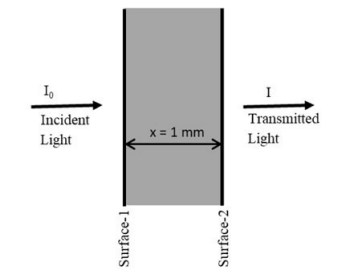
\includegraphics[width=0.5\columnwidth]{figs/ass4_c_q17.png}
    \caption{}
    \label{fig:placeholder}
\end{figure}

(GATE XE 2020)

\item Fe$_3$O$_4$ (also represented as FeO.Fe$_2$O$_3$) is a FCC structured inverse spinel (AB$_2$O$_4$) material where $1/8$ of tetrahedral sites are occupied by half of B cations and $1/2$ of the octahedral sites are occupied by remaining B and A cations. The magnetic moments of cations on octahedral sites are antiparallel with respect to those on tetrahedral sites. Atomic number of Fe is $26$ and that of O is $8$. The saturation magnetic moment of Fe$_3$O$_4$ per formula unit in terms of Bohr magnetons ($\mu_B$) will be \_\_\_\_\_ $\mu_B$. Ignore contribution from orbital magnetic moments.  

(GATE XE 2020)

\item A piezoelectric ceramic with piezoelectric coefficient ($d_{32}$) value of $100 \times 10^{-12} \,\text{C.N}^{-1}$ is subjected to a force, $F_z$, of $10 \,\text{N}$, applied normal to its x–y face, as shown in the figure. If relative dielectric constant ($\varepsilon_r$) of the material is $1100$, the voltage developed along the z-direction of the sample will be \_\_\_\_\_ Volts (round-off to two decimal places). Ignore any nonlinear effects.  

Given: Permittivity of free space ($\varepsilon_0$) $= 8.85 \times 10^{-12}\,\text{F.m}^{-1}$.  

\begin{figure}[H]
    \centering
    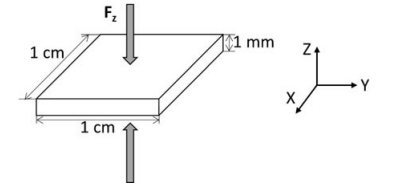
\includegraphics[width=0.5\columnwidth]{figs/ass4_c_q19.png}
    \caption{}
    \label{fig:placeholder}
\end{figure}

(GATE XE 2020)

\item Silicon carbide (SiC) particles are added to Aluminum (Al) matrix to fabricate particle reinforced Al-SiC composite. The resulting composite is required to possess specific modulus ($E/\rho$; $E$: elastic modulus, $\rho$: density) three times that of pure Al. Assuming iso-strain condition, the volume fraction of SiC particles in the composite will be \_\_\_\_\_ (round-off to two decimal places).

\begin{table}[H]
\centering
\begin{tabular}{|c|c|c|}
\hline
Material & $E$ (GPa) & $\rho$ (g.cm$^{-3}$) \\
\hline
Al   & 69  & 2.70 \\
SiC  & 379 & 2.36 \\
\hline
\end{tabular}
\caption{}
\label{}
\end{table}

(GATE XE 2020)

\item Isothermal weight gain per unit area ($\Delta W/A$, where $\Delta W$ is the weight gain (in mg) and $A$ is the area (in cm$^2$)) during oxidation of a metal at $600\,^{\circ}\text{C}$ follows parabolic rate law, where, $\Delta W/A = 1.0 \,\text{mg.cm}^{-2}$ after 100 min of oxidation. The $\Delta W/A$ after 500 min at $600\,^{\circ}\text{C}$ will be \_\_\_\_\_ mg.cm$^{-2}$ (round-off to two decimal places).

(GATE XE 2020)

\item A plain carbon steel sample containing 0.1 wt\% carbon is undergoing carburization at $1100\,^{\circ}\text{C}$ in a carbon rich surroundings with fixed carbon content of 1.0 wt\% all the time. The carburization time necessary to achieve a carbon concentration of 0.46 wt\% at a depth of 5 mm at $1100\,^{\circ}\text{C}$ is \_\_\_\_\_ hour (round off to the nearest integer).

Given: Diffusivity of carbon in iron at $1100\,^{\circ}\text{C}$ is $6.0 \times 10^{-11}$ m$^2$.s$^{-1}$ and

\begin{table}[H]
\centering
\begin{tabular}{|c|c|}
\hline
erf($z$) & $z$ \\
\hline
0.56 & 0.55 \\
0.60 & 0.60 \\
0.64 & 0.65 \\
0.68 & 0.70 \\
\hline
\end{tabular}
\caption{}
\label{}
\end{table}

(GATE XE 2020)

\end{enumerate}

\begin{center}
    \textbf{END OF SECTION - C}
\end{center}

\newpage
\begin{center}
    {\Large \textbf{D : SOLID MECHANICS} }
\end{center}

\begin{enumerate}

\item[] \textbf{Q1 - Q9 carry one mark each.}

\item Which of the following statements is true for a body moving on a dry surface under the action of applied forces?

\begin{enumerate}
\item Kinetic-friction force is zero.
\item Kinetic-friction force is equal to the static-friction force.
\item Kinetic-friction force is greater than the static-friction force.
\item Kinetic-friction force is lower than the static-friction force.
\end{enumerate}
(GATE XE 2020)

\item Consider an isotropic material with Young's modulus $E$ and Poisson's ratio $\nu$.The bulk modulus of this material is given by \_\_\_\_\_\_
\begin{enumerate}
\item $\frac{E}{(1-\nu^2)}$
\item $\frac{E}{2(1+\nu)}$
\item $\frac{E}{3(1-2\nu)}$
\item $\frac{E\nu}{(1+\nu)(1-2\nu)}$
\end{enumerate}
(GATE XE 2020)

\item A body subjected to \_\_\_\_\_\_ does not undergo change in volume.
\begin{enumerate}
\item uniform tension
\item pure shear
\item pure bending
\item hydrostatic pressure
\end{enumerate}
(GATE XE 2020)

\item The angular momentum of a particle moving under a central force is
\begin{enumerate}
\item zero
\item constant in both magnitude and direction
\item constant in magnitude but not direction
\item constant in direction but not magnitude
\end{enumerate}
(GATE XE 2020)

\item According to Euler-Bernoulli theory, which of the following statements best describes the state of a beam subjected to pure bending?
\begin{enumerate}
\item Transverse shear stress and transverse shear strain are zero
\item Transverse shear stress is not zero but transverse shear strain is zero
\item Transverse shear stress is zero but transverse shear strain is not zero
\item Transverse shear stress and transverse shear strain are not zero
\end{enumerate}
(GATE XE 2020)

\item A rigid square ABCD is subjected to planar forces at the corners as shown.
\begin{figure}[H]
    \centering
    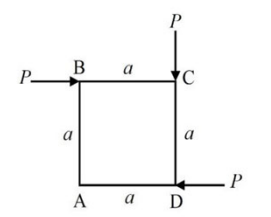
\includegraphics[width=0.5\columnwidth]{figs/ass4_d_q6_1.png}
    \caption{}
    \label{fig:placeholder}
\end{figure}

For this force system, the equivalent force couple system at corner A can be represented as 

\begin{figure}[H]
    \centering
    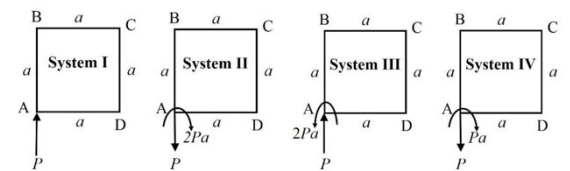
\includegraphics[width=0.8\columnwidth]{figs/ass4_d_q6_2.png}
    \caption{}
    \label{fig:placeholder}
\end{figure}

\begin{enumerate}
\item System I
\item System II
\item System III
\item System IV
\end{enumerate}
(GATE XE 2020)

 \item A particle of mass $0.1\,\text{kg}$, which is released from rest, falls vertically downward under gravity in a fluid. The fluid offers a resistive force, which is linearly proportional to the particle velocity with $0.1\,\text{N}\!\cdot\!\text{s/m}$ as the constant of proportionality. The uniform gravitational acceleration is $10\,\text{m/s}^2$ throughout the trajectory of the particle. The magnitude of the particle velocity (in m/s) at time $1\,\text{s}$ after release (rounded off to two decimal places) is \_\_\_\_\_\_.
 
(GATE XE 2020)

\item The state of two-dimensional plane stress at a point in a body is shown on the triangular element $ABC$, where $\cos\theta=\tfrac{3}{5}$ and $\sin\theta=\tfrac{4}{5}$. The normal stress (in MPa) on the plane $AC$ is \_\_\_\_\_. 

\begin{figure}[H]
    \centering
    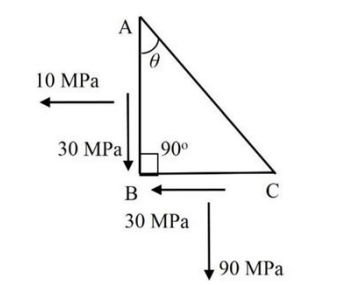
\includegraphics[width=0.5\columnwidth]{figs/ass4_d_q8.png}
    \caption{}
    \label{fig:placeholder}
\end{figure}

(GATE XE 2020)

\item Consider two point masses $m=10\,\text{kg}$ and $M=30\,\text{kg}$ connected by a massless inextensible string passing over a massless and frictionless pulley with radius $a=100\,\text{mm}$ as shown. The masses are released from rest and move vertically under the action of gravity. Let acceleration due to gravity, $g=10\,\text{m/s}^2$. The tension (in N) in the string is \_\_\_\_\_\_. 

\begin{figure}[H]
    \centering
    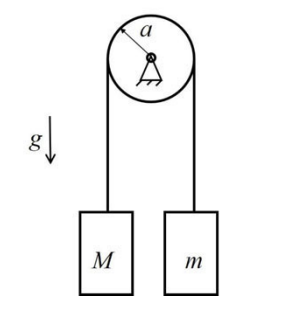
\includegraphics[width=0.5\columnwidth]{figs/ass4_d_q9.png}
    \caption{}
    \label{fig:placeholder}
\end{figure}

(GATE XE 2020)

\item[] \textbf{Q10 - Q22 carry two marks each.}

\item The cantilever beam $AC$ is composed of two segments $AB$ and $BC$ that are rigidly connected at $B$. The flexural rigidity of the segment $AB$ is $EI$, whereas the flexural rigidity of the segment $BC$ is assumed to be infinite. Determine the magnitude of slope at $B$ due to a force $P$ applied at $C$.

\begin{figure}[H]
    \centering
    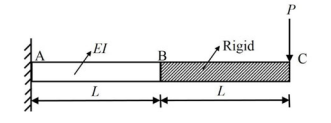
\includegraphics[width=0.5\columnwidth]{figs/ass4_d_q10.png}
    \caption{}
    \label{fig:placeholder}
\end{figure}

\begin{enumerate}
\item $\dfrac{5PL^2}{6EI}$
\item $\dfrac{PL^2}{2EI}$
\item $\dfrac{PL^2}{EI}$
\item $\dfrac{3PL^2}{2EI}$
\end{enumerate}
(GATE XE 2020)

\item Determine the correctness or otherwise of the following Assertion [a] and Reason [r].

Assertion [a]: Efficient columns are designed so that most of the column’s cross-sectional area is located as far away as possible from the principal centroidal axes of the section.  

Reason [r]: Load carrying capacity of columns will increase as the moment of inertia of the cross-section increases.  

\begin{enumerate}
\item Both [a] and [r] are true and [r] is the correct reason for [a].
\item Both [a] and [r] are true but [r] is not the correct reason for [a].
\item Both [a] and [r] are false.
\item [a] is true but [r] is false.
\end{enumerate}
(GATE XE 2020)

\item Consider the structure consisting of two massless elastic bars $AB$ and $BC$, each of length $L$, cross-sectional area $A$, and Young’s modulus $E$. Connections at $A$, $B$, $C$ are all pinned. A horizontal force $P$ acts on the joint $B$ as shown. Calculate the horizontal deflection of the joint $B$.

\begin{figure}[H]
    \centering
    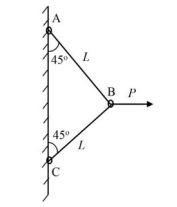
\includegraphics[width=0.5\columnwidth]{figs/ass4_d_q12.png}
    \caption{}
    \label{fig:placeholder}
\end{figure}

\begin{enumerate}
\item $\dfrac{PL}{2AE}$
\item $\dfrac{PL}{AE}$
\item $\dfrac{\sqrt{2}\,PL}{AE}$
\item $\dfrac{PL}{\sqrt{2}AE}$
\end{enumerate}
(GATE XE 2020)

\item A rigid bar $ABC$ of mass $m$ and length $L$ is hinged at $A$ and has a point mass $M$ attached at $C$. An elastic spring with linear stiffness $k$ is attached at $B$ as shown. Ignore the effect of gravity and damping. The natural frequency of small oscillations of this system is \_\_\_\_\_\_.

\begin{figure}[H]
    \centering
    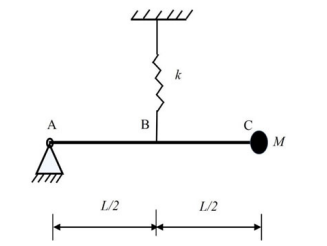
\includegraphics[width=0.5\columnwidth]{figs/ass4_d_q13.png}
    \caption{}
    \label{fig:placeholder}
\end{figure}

\begin{enumerate}
\item $\sqrt{\dfrac{k}{4M+m}}$
\item $\sqrt{\dfrac{k}{2(M+2m)}}$
\item $\sqrt{\dfrac{3k}{3M+m}}$
\item $\sqrt{\dfrac{3k}{4(3M+m)}}$
\end{enumerate}
(GATE XE 2020)

\item A beam of flexural rigidity $EI$ is fixed at $A$ and supported by a linear spring of stiffness $k=\dfrac{EI}{L^{3}}$ at $B$. Determine the compressive force developed in the spring, when the beam is subjected to a uniformly distributed load of $w$ per unit length.  

\begin{figure}[H]
    \centering
    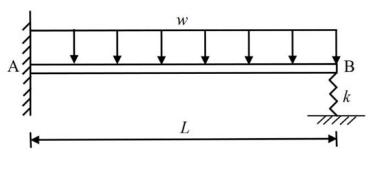
\includegraphics[width=0.5\columnwidth]{figs/ass4_d_q14.png}
    \caption{}
    \label{fig:placeholder}
\end{figure}


\begin{enumerate}
\item $\dfrac{3wL}{32}$
\item $\dfrac{3wL}{16}$
\item $\dfrac{wL}{2}$
\item $\dfrac{wL}{8}$
\end{enumerate}
(GATE XE 2020)

\item The bar $AB$ is fixed at $A$ and is separated by a gap of $0.005 \,\text{mm}$ from wall at $C$ as shown. The temperature of the bar is increased by $10^{\circ}\text{C}$. If the Young’s modulus of the bar is $E=200 \,\text{GPa}$ and the coefficient of thermal expansion is $\alpha = 10 \times 10^{-6}\, /^\circ \text{C}$, then the magnitude of the compressive stress (in MPa) developed in the bar is \_\_\_\_\_\_.

\begin{figure}[H]
    \centering
    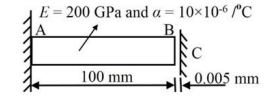
\includegraphics[width=0.5\columnwidth]{figs/ass4_d_q15.png}
    \caption{}
    \label{fig:placeholder}
\end{figure}
(GATE XE 2020)

\item A thin walled spherical pressure vessel has mean radius $100 \,\text{mm}$ and wall thickness $10 \,\text{mm}$. The material has Young's modulus $200 \,\text{GPa}$ and Poisson’s ratio $0.25$. If the internal pressure is $100 \,\text{MPa}$, the radial displacement (in mm) of the spherical pressure vessel (rounded off to two decimal places) is \_\_\_\_\_\_.  

(GATE XE 2020)

\item A particle of mass $m = 100 \,\text{kg}$ is released from rest and falls under gravity through a height of $H = 1 \,\text{m}$ directly onto an upright massless elastic bar of length $L = 200 \,\text{mm}$. Young's modulus $200 \,\text{GPa}$, and cross-sectional area \_\_\_\_\_\_.  
Assume the following during impact:  
(a) particle mass sticks to the bar,  
(b) the bar does not buckle, and  
(c) no energy is lost.  

Use gravitational acceleration $g = 10 \,\text{m/s}^2$.  
The maximum axial compression (in mm) of the bar due to the impact (rounded off to three decimal places) is \_\_\_\_\_\_.  

\begin{figure}[H]
    \centering
    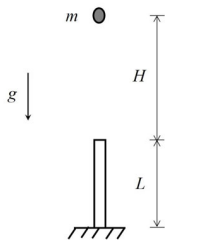
\includegraphics[width=0.5\columnwidth]{figs/ass4_d_q17.png}
    \caption{}
    \label{fig:placeholder}
\end{figure}

(GATE XE 2020)

\item A pin-jointed truss has a pin support at $A$ and a roller support at $C$. All the members are made of the same material and have the same cross-section. Neglect the self-weight of the members. Due to the applied loading shown, the total number of zero-force members is \_\_\_\_\_\_.  

\begin{figure}[H]
    \centering
    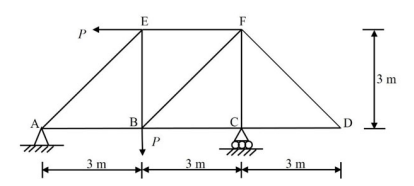
\includegraphics[width=0.5\columnwidth]{figs/ass4_d_q18.png}
    \caption{}
    \label{fig:placeholder}
\end{figure}

(GATE XE 2020)

\item Two beams $AB$ and $BC$ having diameter of $100 \,\text{mm}$ are connected by an internal hinge at $B$. The structure is fixed at $A$ and roller supported at $C$. Load of $P = 1 \,\text{kN}$ is applied at $B$. Ignoring the effect of any transverse shear stress, the tensile stress (in MPa) developed at $A$ due to bending (rounded off to three decimal places) is \_\_\_\_\_\_\_.  

\begin{figure}[H]
    \centering
    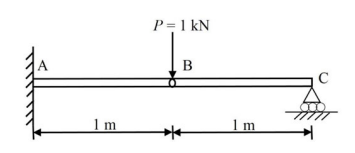
\includegraphics[width=0.5\columnwidth]{figs/ass4_d_q19.png}
    \caption{}
    \label{fig:placeholder}
\end{figure}

(GATE XE 2020)

\item The shear force diagram for a beam $AD$, which is simply supported at $A$ and $D$, is shown. The magnitude of the maximum bending moment (in kN-m) in the beam (rounded off to three decimal places) is \_\_\_\_\_\_\_.  

\begin{figure}[H]
    \centering
    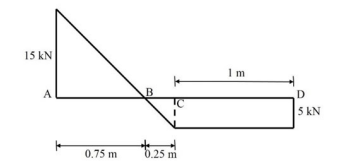
\includegraphics[width=0.5\columnwidth]{figs/ass4_d_q20.png}
    \caption{}
    \label{fig:placeholder}
\end{figure}

(GATE XE 2020)

\item A rectangular thin plate with Young's modulus $200 \,\text{GPa}$ and Poisson's ratio $0.30$ is subjected to uniform stress distribution at its edges as shown. However, it is stated that the dimension $b$ of the plate does not change under the action of the stress components $\sigma_{xx}$ and $\sigma_{yy}$.  

Considering micro-strains (in $10^{-6}$), the change in the length of dimension $a$ (in mm) is \_\_\_\_\_\_ (rounded off to three decimal places).  

\begin{figure}[H]
    \centering
    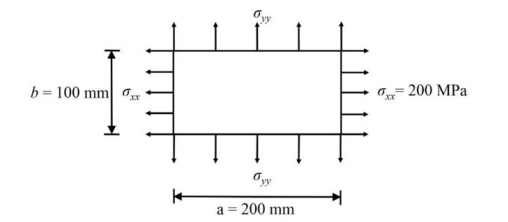
\includegraphics[width=0.5\columnwidth]{figs/ass4_d_q21.png}
    \caption{}
    \label{fig:placeholder}
\end{figure}
(GATE XE 2020)

\item A solid transmission shaft has length $10 \,\text{m}$ and diameter $100 \,\text{mm}$. The shaft is supported by frictionless bearings at the ends that act as simple supports. In addition to its self-weight acting as a uniformly distributed load per unit length, an operational torque of $5\pi \,\text{kN.m}$ is applied.  

The density and yield strength of the material are $8000 \,\text{kg/m}^3$ and $350 \,\text{MPa}$, respectively. Use gravitational acceleration as $10 \,\text{m/s}^2$ and ignore the effect of transverse shear stress.  

The factor of safety of the shaft as per maximum shear stress failure theory (Tresca criterion) is \_\_\_\_\_\_\_ (rounded off to two decimal places). 

(GATE XE 2020)

\end{enumerate}

\begin{center}
    \textbf{END OF SECTION - D}
\end{center}

\newpage
\begin{center}
    {\Large \textbf{E : THERMODYNAMICS} }
\end{center}

\begin{enumerate}

\item[] \textbf{Q1 - Q9 carry one mark each.}
\item If $x$ and $y$ are two independent intensive properties of a thermodynamic system, then which relation among the followings fails to identify $z$ as another thermodynamic property?

\begin{enumerate}
\item $dz = x \, dy + y \, dx$
\item $dz = x \, dy - y \, dx$
\item $dz = 2 \, dy + dx$
\item $dz = \dfrac{dy}{x} + \dfrac{y \, dx}{x^2}$
\end{enumerate}
(GATE XE 2020)

\item Internal energy of a thermodynamic system is defined by the
\begin{enumerate}
\item zeroth law of thermodynamics
\item first law of thermodynamics
\item second law of thermodynamics
\item third law of thermodynamics
\end{enumerate}
(GATE XE 2020)

\item In a polytropic process described by $PV^n = \text{constant}$, if $n=0$, the process is called as
\begin{enumerate}
\item isobaric
\item isochoric
\item isothermal
\item isentropic
\end{enumerate}
(GATE XE 2020)

\item The relation between the coefficient of performance of a refrigerator $(COP)_R$ and the coefficient of performance of a heat pump $(COP)_{HP}$ is
\begin{enumerate}
\item $(COP)_{HP} = (COP)_R + 1$
\item $(COP)_{HP} = (COP)_R - 1$
\item $(COP)_{HP} = 1 - (COP)_R$
\item $(COP)_{HP} \times (COP)_R = 1$
\end{enumerate}
(GATE XE 2020)

\item If $L_1, L_2$ and $L_3$ are the latent heats of vaporization at the critical temperature of nitrogen, water and ammonia, respectively, then which one of the following is true?
\begin{enumerate}
\item $L_1 > L_2 > L_3$
\item $L_1 > L_2$ and $L_2 = L_3$
\item $L_1 < L_2 < L_3$
\item $L_1 = L_2 = L_3$
\end{enumerate}
(GATE XE 2020)

\item A new temperature scale ($^{\circ}N$) has been proposed where the normal freezing and normal boiling points of water are marked as $500\,^{\circ}N$ and $100\,^{\circ}N$, respectively. If the temperature of a system is measured to be $0\,^{\circ}N$, its temperature according to the Celsius scale (in $^{\circ}C$) is \_\_\_\_\_\_\_  

(GATE XE 2020)

\item Let $Z_1$ represent the compressibility factor of air at $2 \,\text{bar}$ and $600 \,\text{K}$, and $Z_2$ represent the compressibility factor of air at $1 \,\text{bar}$ and $300 \,\text{K}$. If air is assumed to be an ideal gas having gas constant of $0.287 \,\text{kJ/kg.K}$, then $Z_1/Z_2$ is \_\_\_\_\_\_\_  

(GATE XE 2020)

\item The rate of heat received by a heat engine from a source at $900 \,\text{K}$ is $600 \,\text{kJ/s}$. The engine rejects heat to the sink at $300 \,\text{K}$. The heat engine produces a power of $200 \,\text{kW}$. The irreversibility rate (in kW) of the process is \_\_\_\_\_\_\_  

(GATE XE 2020)

\item An engine working on the air standard Diesel cycle has a compression ratio of $18$. The cycle has a cut-off ratio of $1.7$. If the ratio of specific heats of air is $1.4$, then the thermal efficiency (in \%) of the cycle (rounded off to $1$ decimal place) is \_\_\_\_\_\_\_  

(GATE XE 2020)

\item[] \textbf{Q10 - Q22 carry two marks each.}
\item A system with rigid walls is initially at a temperature of $T_1$. It is used as the heat source for a heat engine, which rejects heat to a reservoir maintained at $T_0$ ($T_0 < T_1$). The specific heats of the system are constant. If the temperature of the system finally reduces to $T_0$, then the maximum work recoverable from the heat engine per unit mass of the system is
\begin{enumerate}
\item $c_v \left[ (T_1 - T_0) - T_0 \ln \left( \dfrac{T_1}{T_0} \right) \right]$
\item $c_v (T_1 - T_0)$
\item $c_v T_0 \ln \left( \dfrac{T_1}{T_0} \right)$
\item $c_v \dfrac{T_1^2}{T_0}$
\end{enumerate}
(GATE XE 2020)

\item A reversible heat engine is operating between two reservoirs maintained at $T_1$ and $T_2$, where $T_1 > T_2$. Which one of the following is the most effective option for increasing its thermal efficiency?
\begin{enumerate}
\item increasing $T_1$, while keeping $T_2$ constant
\item decreasing $T_1$, while keeping $T_2$ constant
\item increasing $T_2$, while keeping $T_1$ constant
\item decreasing $T_2$, while keeping $T_1$ constant
\end{enumerate}
(GATE XE 2020)

\item A $4\text{ m}^3$ reservoir contains $10 \,\text{kg}$ of a real gas at $200 \,\text{K}$. If this gas follows the van der Waal’s equation of state with $a = 0.0687 \,\text{m}^6 \,\text{kPa}/\text{kg}^2$, $b = 0.00657 \,\text{m}^3/\text{kg}$ and $R = 0.187 \,\text{kJ/kg.K}$, then the reservoir pressure (in kPa) is
\begin{enumerate}
\item 93.5
\item 94.6
\item 95.5
\item 101.3
\end{enumerate}
(GATE XE 2020)

\item Air at a pressure of $86 \,\text{kPa}$ and specific volume of $1 \,\text{m}^3/\text{kg}$ is heated at constant pressure till it reaches $627^\circ \text{C}$. Air is assumed to be an ideal gas with constant specific heats. It has the gas constant of $0.287 \,\text{kJ/kg.K}$ and ratio of specific heats of $1.4$. The change in specific entropy of air (in kJ/kg.K) during this process will be
\begin{enumerate}
\item 1.104
\item 0.740
\item 0.788
\item 0.529
\end{enumerate}
(GATE XE 2020)

\item An air standard Otto cycle has compression ratio of 4. The compression ratio of this cycle is changed to 6. If the ratio of specific heats is $1.4$, the percentage increase in its thermal efficiency will be
\begin{enumerate}
\item 20.2
\item 27.2
\item 42.6
\item 51.2
\end{enumerate}
(GATE XE 2020)

\item In a mixture of gas there are $0.1$ kmol of oxygen ($O_2$), $0.1$ kmol of nitrogen ($N_2$) and $0.8$ kmol of methane ($CH_4$). If the molar mass of $O_2$, $N_2$ and $CH_4$ are $32 \,\text{kg/kmol}$, $28 \,\text{kg/kmol}$ and $16 \,\text{kg/kmol}$, respectively, then the mass fraction of $N_2$ in the gas mixture is
\begin{enumerate}
\item 0.100
\item 0.170
\item 0.148
\item 0.680
\end{enumerate}
(GATE XE 2020)

\item A particular gas sample is initially maintained at $6000 \,\text{cm}^3$ and $100 \,\text{kPa}$. 
It is compressed during a quasistatic process following the relation $PV^2 = \text{constant}$. 
The compression continues till the volume becomes $2000 \,\text{cm}^3$. 
The magnitude of the corresponding work transfer (in kJ) (rounded off to 2 decimal places) is 
\_\_\_\_\_\_\_ 

(GATE XE 2020)

\item Carbon dioxide (CO$_2$) enters an adiabatic rigid nozzle steadily at $1 \,\text{MPa}$ and $500^\circ \text{C}$ with a mass flow rate of $1.5 \,\text{kg/s}$. 
The inlet area of the nozzle is $40 \,\text{cm}^2$ and the exit velocity is 10 times that of the inlet. 
If CO$_2$ can be considered as an ideal gas with gas constant of $0.19 \,\text{kJ/kg.K}$ and the ratio of specific heats of $1.29$, the exit temperature (in K) (rounded off to 1 decimal place) is 
\_\_\_\_\_\_\_ 

(GATE XE 2020)

\item A closed system containing $8 \,\text{kg}$ of gas undergoes an expansion process following the relation $PV^{1.2} = \text{constant}$. 
The initial and final pressures are $1 \,\text{MPa}$ and $5 \,\text{kPa}$, respectively, while the initial volume is $1 \,\text{m}^3$. 
If the specific internal energy of the gas decreases by $40 \,\text{kJ/kg}$ during the process, the heat transfer (in kJ) associated with the process (rounded off to 1 decimal place) is 
\_\_\_\_\_\_\_ 

(GATE XE 2020)

\item Saturation pressure of water at $5^\circ \text{C}$ is $0.8725 \,\text{kPa}$. 
If the latent heat of vaporization is $2489.1 \,\text{kJ/kg}$ and gas constant is $0.4615 \,\text{kJ/kg.K}$, then the saturation pressure at $10^\circ \text{C}$ (in kPa) (rounded off to 2 decimal places) is 
\_\_\_\_\_\_\_ 

(GATE XE 2020)

\item The turbine inlet conditions of a Rankine cycle are $10 \,\text{MPa}$ and $500^\circ \text{C}$, while the condenser pressure is $10 \,\text{kPa}$. 
The enthalpy and entropy of saturated liquid at $10 \,\text{kPa}$ are $191.8 \,\text{kJ/kg}$ and $0.6492 \,\text{kJ/kg.K}$, respectively, while the enthalpy and entropy of vaporization at $10 \,\text{kPa}$ are $2392.1 \,\text{kJ/kg}$ and $7.4996 \,\text{kJ/kg.K}$, respectively. 
The enthalpy and entropy at the inlet to the turbine are $3375.1 \,\text{kJ/kg}$ and $6.5995 \,\text{kJ/kg.K}$, respectively. 
The condenser outlet has saturated liquid. Neglecting the pump work, the thermal efficiency (in \%) of the cycle (rounded off to 1 decimal place) is 
\_\_\_\_\_\_\_ 

(GATE XE 2020)

\item The minimum and maximum temperatures of an air standard Brayton cycle are $300 \,\text{K}$ and $1100 \,\text{K}$, respectively. 
The pressure ratio of this cycle is $6$. 
The ratio of specific heats is $1.4$ and the specific heats are constant. 
For this cycle, the ratio of network output to the turbine work (rounded off to 2 decimal places) is 
\_\_\_\_\_\_\_ 

(GATE XE 2020)

\item The specific humidity of air at $100 \,\text{kPa}$ is $0.015 \,\text{kg}$ of vapour per kg of dry air. 
The partial pressure of vapour (in kPa) in the existing state (rounded off to 2 decimal places) is 
\_\_\_\_\_\_\_ 

(GATE XE 2020)

\end{enumerate}

\begin{center}
    \textbf{END OF SECTION - E}
\end{center}

\newpage
\begin{center}
    {\Large \textbf{F : POLYMER SCIENCE AND ENGINEERING} }
\end{center}

\begin{enumerate}

\item[] \textbf{Q1 - Q9 carry one mark each.}
\item The solvent in which chain transfer is maximum in a radical polymerization is  
\begin{enumerate}
\item Benzene  
\item Chloroform  
\item Carbon tetrachloride  
\item Toluene  
\end{enumerate}  
(GATE XE 2020)

\item The monomer that can NOT be polymerized by anionic polymerization is  
\begin{enumerate}
\item Styrene  
\item Ethyl vinyl ether  
\item Butadiene  
\item Methyl methacrylate  
\end{enumerate}  
(GATE XE 2020)

\item The elastomer retaining flexibility at the lowest temperature is  
\begin{enumerate}
\item Styrene butadiene rubber  
\item Nitrile rubber  
\item Silicone rubber  
\item Butyl rubber  
\end{enumerate}  
(GATE XE 2020)

\item The polymer with minimum number of branches is  
\begin{enumerate}
\item LDPE  
\item LLDPE  
\item HDPE  
\item VLDPE  
\end{enumerate}  
(GATE XE 2020)

\item The nearest value of conductivity of Nylon 6 is  
\begin{enumerate}
\item $10^6 \,\text{S/m}$  
\item $10^5 \,\text{S/m}$  
\item $10^{-13} \,\text{S/m}$  
\item $10^{-21} \,\text{S/m}$  
\end{enumerate}  
(GATE XE 2020)

\item Aramid is a  
\begin{enumerate}
\item Polyamide  
\item Polyether  
\item Polyester  
\item Polyimide  
\end{enumerate}  
(GATE XE 2020)

\item A miscible blend in 1:1 (by weight) composition is formed with  
\begin{enumerate}
\item Polystyrene and polybutadiene  
\item Polystyrene and poly(phenylene oxide)  
\item Polystyrene and poly(methyl methacrylate)  
\item Polystyrene and poly(dimethyl siloxane)  
\end{enumerate}  
(GATE XE 2020)

\item Dicumyl peroxide is a  
\begin{enumerate}
\item Plasticizer  
\item Cross-linking agent  
\item Mold release agent  
\item Peptizer  
\end{enumerate}  
(GATE XE 2020)

\item The change in stress of a polymer as a function of time at a fixed strain is known as  
\begin{enumerate}
\item Fatigue  
\item Creep  
\item Stress relaxation  
\item Fracture toughness  
\end{enumerate}  
(GATE XE 2020)

\item[] \textbf{Q10 - Q22 carry two marks each.}
\item Match the polymers in Column A with their corresponding polymerization methods in Column B.

\begin{table}[H]
\centering
\caption{}
\label{}
\begin{tabular}{|l|l|}
\hline
\textbf{Column A} & \textbf{Column B} \\ \hline
P\; Bisphenol A polycarbonate & 1\; Cationic \\ \hline
Q\; Polyethylene               & 2\; Step-growth \\ \hline
R\; Poly(styrene-\!b-\!butadiene) & 3\; Coordination \\ \hline
S\; Butyl rubber              & 4\; Anionic \\ \hline
\end{tabular}
\end{table}

\begin{enumerate}
\item  P-3, Q-2, R-4, S-1
\item  P-4, Q-3, R-2, S-1
\item  P-2, Q-3, R-4, S-1
\item  P-1, Q-3, R-4, S-2
\end{enumerate}

(GATE XE 2020)

\item Match the appropriate processing technique in Column A to fabricate the product in Column B.

\begin{table}[H]
\centering
\caption{}
\label{}
\begin{tabular}{|l|l|}
\hline
\textbf{Column A} & \textbf{Column B} \\ \hline
P\; Blow molding         & 1\; Plastic buckets \\ \hline
Q\; Rotational molding   & 2\; PVC sheet \\ \hline
R\; Injection molding    & 3\; Basket ball \\ \hline
S\; Calendering          & 4\; Plastic bottles \\ \hline
\end{tabular}
\end{table}

\begin{enumerate}
\item  P-2, Q-3, R-4, S-1
\item  P-3, Q-4, R-2, S-1
\item  P-4, Q-2, R-1, S-3
\item  P-4, Q-3, R-1, S-2
\end{enumerate}

(GATE XE 2020)

\item Match the appropriate characterization technique in Column A used to determine the polymer attributes in Column B.

\begin{table}[H]
\centering
\caption{} \label{}
\begin{tabular}{|l|l|}
\hline
\textbf{Column A} & \textbf{Column B} \\ \hline
P\; Gel permeation chromatography & 1\; Functional group \\ \hline
Q\; FT-IR spectroscopy            & 2\; Crystal structure \\ \hline
R\; Differential scanning calorimetry & 3\; Glass transition temperature \\ \hline
S\; X-ray diffraction             & 4\; Molecular weight \\ \hline
\end{tabular}
\end{table}

\begin{enumerate}
\item P-2, Q-3, R-4, S-1  
\item P-3, Q-4, R-1, S-2  
\item P-2, Q-4, R-1, S-3  
\item P-4, Q-1, R-3, S-2  
\end{enumerate}

(GATE XE 2020)

\item Match each additive in Column A with its function given in Column B.

\begin{table}[H]
\centering
\caption{} \label{}
\begin{tabular}{|l|l|}
\hline
\textbf{Column A} & \textbf{Column B} \\ \hline
P\; Azodiformamide             & 1\; Curing agent \\ \hline
Q\; Di-octyl phthalate         & 2\; UV stabilizer \\ \hline
R\; Benzoyl peroxide           & 3\; Blowing agent \\ \hline
S\; 2-(2$'$-hydroxy phenyl)benzotriazole & 4\; Plasticizer \\ \hline
\end{tabular}
\end{table}

\begin{enumerate}
\item P-2, Q-3, R-1, S-2  
\item P-3, Q-4, R-1, S-2  
\item P-4, Q-3, R-2, S-1  
\item P-1, Q-3, R-4, S-2  
\end{enumerate}

(GATE XE 2020)

\item Plot of shear stress against shear rate for various types of fluids is given below.  
The appropriate assignment for P, Q, R and S is \_\_\_\_\_.  

\begin{figure}[H]
    \centering
    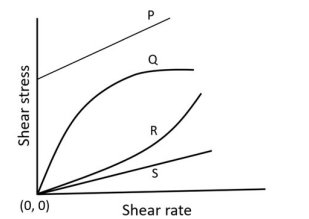
\includegraphics[width=0.5\columnwidth]{figs/ass4_f_q14.png}
    \caption{}
    \label{fig:placeholder}
\end{figure}

\begin{enumerate}
\item P-Dilatant, Q-Bingham plastic, R-Pseudoplastic, S-Newtonian  
\item P-Bingham plastic, Q-Pseudoplastic, R-Dilatant, S-Newtonian  
\item P-Pseudoplastic, Q-Bingham plastic, R-Newtonian, S-Dilatant  
\item P-Newtonian, Q-Dilatant, R-Pseudoplastic, S-Bingham plastic  
\end{enumerate}

(GATE XE 2020)

\item The number average molecular weight of a polyester formed from equimolar mixture of adipic acid and ethylene glycol at a conversion of 99.5\% will be \_\_\_\_\_ (round off to nearest integer).  

(GATE XE 2020)

\item For a freely jointed linear polyethylene chain with molar mass of $1.4\times 10^{5}$ g mol$^{-1}$, the value of root mean square end-to-end distance in nanometer is \_\_\_\_\_ (round off to 1 decimal place). [Given: C–C bond length = 0.154 nanometer]  

(GATE XE 2020)

\item Viscosity measurements were performed for a set of PMMA solutions of different concentrations in toluene at 25$^\circ$C. The plot of reduced viscosity against concentration ($c$) of the PMMA solutions produced an intercept of 21.0 cm$^3$ g$^{-1}$ on the ordinate at $c=0$. The value of viscosity average molecular weight of PMMA in toluene at 25$^\circ$C is \_\_\_\_\_ (round off to nearest integer). [Given: Mark–Houwink constants $K=7.5\times10^{-3}$ cm$^3$ g$^{-1}$ and $a=0.72$ for PMMA in toluene at 25$^\circ$C]  

(GATE XE 2020)

\item Glass fibre reinforced PP composite is to be prepared with 20 volume \% of glass fibre. The densities of glass fibre and PP are 2540 kg m$^{-3}$ and 900 kg m$^{-3}$, respectively. The mass of glass fibre required to produce 1 kg of the composite in kg is \_\_\_\_\_ (round off to 2 decimal places).  

(GATE XE 2020)

\item A polymer solution flows through a cylindrical tube with a diameter of 4 mm at a volumetric flow rate of $10^{-8}$ m$^3$/s. Under laminar flow condition and assuming the polymer solution to be a Newtonian fluid with viscosity $10^3$ N·s/m$^2$, the value of pressure drop per unit length of the tube in N/m$^3$ is \_\_\_\_\_ (round off to nearest integer). [Consider the value of $\pi$ as 3.14]  

(GATE XE 2020)

\item A molten polymer with a bulk modulus of 1 GPa is pressurized to 200 MPa during injection molding. The fractional decrease in volume of the molten polymer at this pressurized condition is \_\_\_\_\_ (round off to 4 decimal places).  

(GATE XE 2020)

\item Assume that each cross-link produced by vulcanization of polyisoprene contains an average of two sulphur atoms and that the sulphur is present only in the cross-links. If 40\% of the isoprene units are cross-linked, the sulphur content in weight percentage is \_\_\_\_\_ (round off to 2 decimal places).  

(GATE XE 2020)

\item A tensile force of 160 N is applied to a piece of vulcanized rubber of dimension 30 mm $\times$ 4 mm $\times$ 4 mm. Assuming the vulcanized rubber to be incompressible, if the sample is elongated to 150\% of its original length under the same applied force, the true stress in N/mm$^2$ will be \_\_\_\_\_ (round off to 1 decimal place).  

(GATE XE 2020)

\end{enumerate}

\begin{center}
    \textbf{END OF SECTION - F}
\end{center}

\newpage
\begin{center}
    {\Large \textbf{G : FOOD TECHNOLOGY} }
\end{center}

\begin{enumerate}

\item[] \textbf{Q1 - Q9 carry one mark each.}
\item The enzyme majorly involved in postmortem degradation of muscle proteins is
\begin{enumerate}
\item Trypsin
\item Calpain
\item Transglutaminase
\item Pepsin
\end{enumerate}
(GATE XE 2020)

\item Which of the following is the correct pair of essential fatty acids?
\begin{enumerate}
\item Oleic acid and Lenoleic acid
\item Lenoleic acid and Linolenic acid
\item Linolenic acid and Lauric acid
\item Linolenic acid and Oleic acid
\end{enumerate}
(GATE XE 2020)

\item Nisin A is produced by
\begin{enumerate}
\item \textit{Aspergillus niger}
\item \textit{Acetobacter aceti}
\item \textit{Lactobacillus lactis}
\item \textit{Clostridium perfringens}
\end{enumerate}
(GATE XE 2020)

\item Which of the following bacteria will stain purple color after Gram staining?
\begin{enumerate}
\item \textit{Bacillus subtilis}
\item \textit{Escherichia coli}
\item \textit{Pseudomonas aeruginosa}
\item \textit{Yersinia pestis}
\end{enumerate}
(GATE XE 2020)

\item The enzyme system used for removal of glucose from egg white prior to its drying consists of
\begin{enumerate}
\item Glucose oxidase and Catalase
\item Glucosidase and Glucoisomerase
\item Glucoisomerase and Catalase
\item Glucoamylase and Glucose oxidase
\end{enumerate}
(GATE XE 2020)

\item The \textbf{INCORRECT} pair of food borne illness and its causative microorganism is
\begin{enumerate}
\item Brucellosis — \textit{Brucella} sp.
\item Peptic ulcers — \textit{Bacillus subtilis}
\item Bubonic plague — \textit{Yersinia pestis}
\item Q fever — \textit{Coxiella burnetii}
\end{enumerate}
(GATE XE 2020)

\item Which of the following is commonly used as a preservative in the tomato sauce?
\begin{enumerate}
\item Sodium sulphite
\item Potassium sorbate
\item Potassium sulphite
\item Sodium benzoate
\end{enumerate}
(GATE XE 2020)

\item The velocity of $2.2\,\mu$m diameter fat particles inside a centrifuge, running at $6000$ rpm and $20^{\circ}\mathrm{C}$, is $0.25$ mm s$^{-1}$. The velocity of $1.5\,\mu$m diameter fat particles inside the same centrifuge running at $7500$ rpm and same temperature (round off to 2 decimal places) will be \_\_\_\_\_\_\_ mm s$^{-1}$.  

(GATE XE 2020)

\item The initial population of a bacterial strain increases from $1\times 10^{4}$ cells per mL to $1\times 10^{8}$ cells per mL in $120$ minutes. The generation time for this strain (round off to 2 decimal places) is \_\_\_\_\_\_\_ minutes. 

(GATE XE 2020)

\item[] \textbf{Q10 - Q22 carry two marks each.}
\item Match the protein in \textbf{Column I} with its food source in \textbf{Column II}.
\begin{table}[H]
\centering
\caption{}
\label{}
\begin{tabular}{|c|c|}
\hline
Column I & Column II \\
\hline
P. Zein & 1. Soybean \\
Q. Gluten & 2. Maize \\
R. Glycinin & 3. Egg \\
S. Ovalbumin & 4. Wheat \\
\hline
\end{tabular}
\end{table}

\begin{enumerate}
\item P-4, Q-1, R-2, S-3
\item P-4, Q-3, R-1, S-2
\item P-2, Q-3, R-1, S-4
\item P-2, Q-4, R-1, S-3
\end{enumerate}
(GATE XE 2020)

\item Match the carbohydrate in \textbf{Column I} with corresponding enzyme used for its hydrolysis in \textbf{Column II}.
\begin{table}[H]
\centering
\caption{}
\label{}
\begin{tabular}{|c|c|}
\hline
Column I & Column II \\
\hline
P. Pectin & 1. Xylanase \\
Q. Lactose & 2. $\beta$-galactosidase \\
R. Hemicellulose & 3. Polygalacturonase \\
S. Inulin & 4. $\beta$-fructofuranosidase \\
\hline
\end{tabular}
\end{table}

\begin{enumerate}
\item P-3, Q-2, R-1, S-4
\item P-2, Q-4, R-1, S-3
\item P-1, Q-2, R-3, S-4
\item P-4, Q-3, R-1, S-2
\end{enumerate}
(GATE XE 2020)

\item Match the edible oil refining stage in \textbf{Column I} with its purpose in \textbf{Column II}.
\begin{table}[H]
\centering
\caption{}
\label{}
\begin{tabular}{|c|c|}
\hline
Column I & Column II \\
\hline
P. Degumming & 1. Separation of triglycerides \\
Q. Neutralization & 2. Removal of pigments \\
R. Bleaching & 3. Removal of phosphatides \\
S. Winterization & 4. Removal of free fatty acids \\
\hline
\end{tabular}
\end{table}

\begin{enumerate}
\item P-3, Q-1, R-2, S-4
\item P-1, Q-4, R-2, S-3
\item P-4, Q-3, R-1, S-2
\item P-3, Q-4, R-2, S-1
\end{enumerate}
(GATE XE 2020)

\item Match the food material in \textbf{Column I} with its related term in \textbf{Column II}.
\begin{table}[H]
\centering
\caption{}
\label{}
\begin{tabular}{|c|c|}
\hline
Column I & Column II \\
\hline
P. Coffee & 1. Wort \\
Q. Cocoa & 2. Must \\
R. Beer & 3. \textit{Arabica} \\
S. Wine & 4. \textit{Theobroma} \\
\hline
\end{tabular}
\end{table}

\begin{enumerate}
\item P-4, Q-2, R-1, S-3
\item P-3, Q-4, R-1, S-2
\item P-3, Q-4, R-2, S-1
\item P-1, Q-3, R-4, S-2
\end{enumerate}
(GATE XE 2020)

\item Match the component/system in \textbf{Column I} with the peeling method for fruits and vegetables in \textbf{Column II}.
\begin{table}[h!]
\centering
\caption{}
\label{}
\begin{tabular}{|c|c|}
\hline
Column I & Column II \\
\hline
P. Lye solution & 1. Flash peeling \\
Q. Carborundum rollers & 2. Flame peeling \\
R. Pressure vessel & 3. Abrasion peeling \\
S. Conveyor belt & 4. Caustic peeling \\
\hline
\end{tabular}
\end{table}

\begin{enumerate}
\item P-4, Q-3, R-2, S-1
\item P-3, Q-4, R-1, S-2
\item P-4, Q-3, R-1, S-2
\item P-3, Q-4, R-2, S-1
\end{enumerate}
(GATE XE 2020)

\item Which among the given options correctly explains the nature of the microbial culture represented by curves 1, 2 and 3 in the following figure?

\begin{figure}[H]
    \centering
    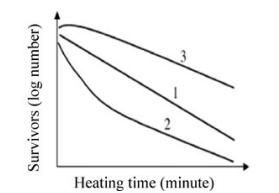
\includegraphics[width=0.5\columnwidth]{figs/ass4_g_q15.png}
    \caption{}
    \label{fig:placeholder}
\end{figure}

\begin{enumerate}
\item 
1. Germination of spores 

2. Homogeneous population 

3. Mixed population of spores and vegetative cells

\item 
1. Homogeneous population 

2. Mixed population of heat sensitive and heat resistant microbes 

3. Germination of spores

\item 
1. Composite population 

2. Spores activated by short exposure to heat 

3. Thermo sensitive and thermo resistant microbes

\item 
1. Mixed population 

2. Microorganisms activated by short exposure to heat 

3. Germination of spores
\end{enumerate}
(GATE XE 2020)

\item Match the equation/law in \textbf{Column I} with its application in \textbf{Column II}.
\begin{table}[H]
\centering
\caption{}
\label{}
\begin{tabular}{|l|l|}
\hline
Column I & Column II \\
\hline
P. Planck's equation & 1. Terminal velocity \\
Q. Arrhenius equation & 2. Freezing time \\
R. Guggenheim--Anderson--de Boer equation & 3. Activation energy \\
S. Stokes' law & 4. Monolayer moisture content \\
\hline
\end{tabular}
\end{table}

\begin{enumerate}
\item P-1, Q-3, R-4, S-2
\item P-2, Q-3, R-1, S-4
\item P-2, Q-3, R-4, S-1
\item P-4, Q-3, R-1, S-2
\end{enumerate}
(GATE XE 2020)

\item Match the absorber used in modified atmosphere packaging and storage in \textbf{Column I} with the scavenger in \textbf{Column II}.
\begin{table}[H]
\centering
\caption{}
\label{}
\begin{tabular}{|l|l|}
\hline
Column I & Column II \\
\hline
P. Oxygen absorber  & 1. Calcium chloride \\
Q. Carbon dioxide absorber & 2. Magnesium oxide \\
R. Ethylene absorber & 3. Ferric oxide \\
S. Moisture absorber & 4. Potassium permanganate \\
\hline
\end{tabular}
\end{table}

\begin{enumerate}
\item P-3, Q-2, R-4, S-1
\item P-1, Q-2, R-4, S-3
\item P-2, Q-3, R-4, S-1
\item P-3, Q-2, R-1, S-4
\end{enumerate}
(GATE XE 2020)

\item During extrusion cooking, food materials are generally subjected to a combination of
\begin{enumerate}
\item high shear and low pressure
\item high temperature and high shear
\item low shear and high temperature
\item low shear and low pressure
\end{enumerate}
(GATE XE 2020)

\item The whole milk at $22^{\circ}\mathrm{C}$ is pumped through a stainless steel pipe at a flow rate of $3\ \mathrm{L\,s^{-1}}$. The length and inner diameter of the pipe are $40\ \mathrm{m}$ and $4\ \mathrm{cm}$, respectively. If viscosity and density of the milk at the pumping temperature are $0.2\ \mathrm{Pa\,s}$ and $1032\ \mathrm{kg\,m^{-3}}$, respectively, the Reynolds number (rounded off to nearest integer) will be \_\_\_\_\_.  

(GATE XE 2020)

\item A hammer mill, operating at a feed rate of $108\ \mathrm{ton\,h^{-1}}$, consumes $10\ \mathrm{kW}$ power for reducing size of wheat grain from $3.92\ \mathrm{mm}$ to $1.25\ \mathrm{mm}$. If Bond's law holds good, the feed rate (round off to $2$ decimal places) for reducing the size of the wheat grain to $0.75\ \mathrm{mm}$ at the same power consumption level is \_\_\_\_\_ $\mathrm{ton\,h^{-1}}$.  

(GATE XE 2020)

\item During spray drying of a milk sample, inlet and outlet temperatures are maintained at $132^{\circ}\mathrm{C}$ and $80^{\circ}\mathrm{C}$, respectively. If the ambient temperature is $29^{\circ}\mathrm{C}$, the thermal efficiency (round off to $2$ decimal places) of the dryer will be \_\_\_\_\_ \%. 

(GATE XE 2020)

\item An orange juice flowing at $0.80\ \mathrm{kg\,s^{-1}}$ enters a counter-current double pipe heat exchanger at $20^{\circ}\mathrm{C}$ and leaves at $72^{\circ}\mathrm{C}$. Inlet and outlet temperatures of the hot water used as heating medium in the exchanger are $81^{\circ}\mathrm{C}$ and $74^{\circ}\mathrm{C}$, respectively. The specific heat of the orange juice is $3.74\ \mathrm{kJ\,kg^{-1}\,K^{-1}}$ and overall heat transfer coefficient is $492\ \mathrm{W\,m^{-2}\,K^{-1}}$. The heat transfer surface area (round off to $2$ decimal places) will be \_\_\_\_\_ $\mathrm{m^{2}}$.  

(GATE XE 2020)

\end{enumerate}

\begin{center}
    \textbf{END OF SECTION - G}
\end{center}

\newpage
\begin{center}
    {\Large \textbf{H : ATMOSPHERIC AND OCEANIC SCIENCES} }
\end{center}

\begin{enumerate}

\item[] \textbf{Q1 - Q9 carry one mark each.}
\item In the northern hemisphere, the flow in the middle depths of the ocean is geostrophic. As we go down from that level and start approaching the bottom of the ocean, the flow deflects to the left of the geostrophic current because
\begin{enumerate}
\item friction decreases and Coriolis force increases
\item friction decreases and Coriolis force decreases
\item friction increases and Coriolis force increases
\item friction increases and Coriolis force decreases
\end{enumerate}
(GATE XE 2020)

\item Which one of the following is the definition of a monsoon?
\begin{enumerate}
\item Seasonal reversal of wind direction
\item High rainfall
\item Occurs in the summer
\item Occurs in the tropics
\end{enumerate}
(GATE XE 2020)

\item Anthropogenic emission of \_\_\_\_\_ is the main contributor to the ongoing ocean acidification.
\begin{enumerate}
\item Methane
\item Carbon dioxide
\item Nitrous oxide
\item Sulphuric acid
\end{enumerate}
(GATE XE 2020)

\item What are phytoplankton?
\begin{enumerate}
\item Microscopic animal life floating on surface of water bodies
\item Pollen floating freely on surface of water bodies
\item Microscopic plant life floating on surface of water bodies
\item Microscopic plant life living on the floor of water bodies
\end{enumerate}
(GATE XE 2020)

\item Consider the two atmospheric virtual temperature profiles observed in Delhi given in Figures (i) and (ii).  

\begin{figure}[H]
    \centering
    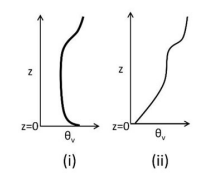
\includegraphics[width=0.5\columnwidth]{figs/ass4_h_q5.png}
    \caption{}
    \label{fig:placeholder}
\end{figure}

At what times of the day are you most likely to see such profiles?  
\begin{enumerate}
\item (i) Midnight and (ii) noon
\item (i) 3 pm and (ii) 3 am
\item (i) Sunrise and (ii) sunset
\item (i) 3 am and (ii) 3 pm
\end{enumerate}
(GATE XE 2020)

\item A south-easterly wind is blowing towards which direction?
\begin{enumerate}
\item 135$^{\circ}$
\item 157.5$^{\circ}$
\item 315$^{\circ}$
\item 252$^{\circ}$
\end{enumerate}
(GATE XE 2020)

\item Consider a dry parcel of 30$^{\circ}$C in an isothermal environment at 25$^{\circ}$C. The parcel rises adiabatically by 1 km. Assuming $g=10\ \mathrm{ms^{-2}}$ and air density $=1\ \mathrm{kgm^{-3}}$, the buoyancy force at the new location (rounded off to 2 decimal places) is \_\_\_\_\_.  

(GATE XE 2020)

\item The emissivity of polluted air dust reflects and transmits 20\% and 60\% of the incoming solar radiation, respectively, at a given wavelength (correct up to 1 decimal place). The absorptivity is \_\_\_\_\_.  

(GATE XE 2020)

\item Given that the angular velocity of rotation of the Earth = $7.3 \times 10^{-5}\ \mathrm{s^{-1}}$, the period of inertial oscillations generated in the oceans by surface winds at 30$^{\circ}$N latitude (rounded off to the nearest integer) is \_\_\_\_\_ hours.  

(GATE XE 2020)

\item[] \textbf{Q10 - Q22 carry two marks each.}
\item Consider a high pressure centre in the northern hemisphere with tangential winds of 10 m s$^{-1}$ at a distance of 500 km from the centre. Assuming solid body rotation principles, what is the relative vorticity of the flow?
\begin{enumerate}
\item $2 \times 10^{-5}\ \mathrm{s^{-1}}$
\item $-2 \times 10^{-5}\ \mathrm{s^{-1}}$
\item $4 \times 10^{-5}\ \mathrm{s^{-1}}$
\item $-4 \times 10^{-5}\ \mathrm{s^{-1}}$
\end{enumerate}
(GATE XE 2020)

\item Which one of the following statements is true for atmospheric and oceanic general circulation models?
\begin{enumerate}
\item Vertical velocity is ignored in oceanic models but not in atmospheric models.
\item Boussinesq approximation is adequate in oceanic models but not in atmospheric models.
\item Atmospheric models need a longer spin-up and integration time than oceanic models.
\item Atmospheric models need parameterizations for subgrid scale processes but oceanic models do not.
\end{enumerate}
(GATE XE 2020)

\item Consider a scenario where air temperature increases by 2$^\circ$C. We know that saturation vapour pressure for water increases with temperature. As a result of this effect, the water vapour content of the atmosphere will \_\_\_\_\_\_\_ and the net warming will be \_\_\_\_\_\_\_ than 2$^\circ$C. The correct pair of words to fill in the blanks (in the right order) is
\begin{enumerate}
\item increase, more
\item increase, less
\item decrease, more
\item decrease, less
\end{enumerate}
(GATE XE 2020)

\item The prevailing Trade winds over the Equator in the Pacific Ocean result in piling up of waters in the \_\_\_\_\_\_\_ part of the ocean. As a result, the gradients of the thermocline and the ocean surface have \_\_\_\_\_\_\_ signs. The correct pair of words to fill in the blanks (in the right order) is
\begin{enumerate}
\item western, opposite
\item western, same
\item eastern, opposite
\item eastern, same
\end{enumerate}
(GATE XE 2020)

\item Consider two different cases, shown in Figures (i) and (ii), with two layers of water of same density on top of each other.  

\begin{figure}[H]
    \centering
    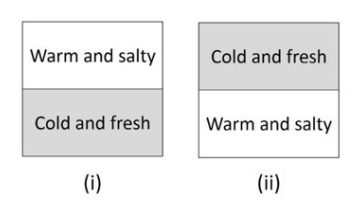
\includegraphics[width=0.5\columnwidth]{figs/ass4_h_q14.png}
    \caption{}
    \label{fig:placeholder}
\end{figure}

Which one of the following statements is true about convective plumes across the interface of the two layers?  
\begin{enumerate}
\item Upward convective plumes in (i) and downward convective plumes in (ii)  
\item Downward convective plumes in (i) and upward convective plumes in (ii)  
\item No convective plume in (i) and (ii)  
\item No convective plume in (i) but upward convective plumes in (ii)  
\end{enumerate}
(GATE XE 2020)

\item During the Indian summer monsoon, surface outgoing longwave radiation (OLR) over the Arabian Sea is often observed to be low because
\begin{enumerate}
\item monsoon winds advect the OLR away into the Indian subcontinent  
\item monsoon clouds limit incoming solar radiation  
\item surface Bowen ratio is low  
\item enhanced convection  
\end{enumerate}
(GATE XE 2020)

\item A tsunami wave in the ocean is approaching the coast. Assuming $g = 10$ m s$^{-2}$, the correct group speed of the wave at a depth of 1 km is
\begin{enumerate}
\item 1 m s$^{-1}$
\item 10 m s$^{-1}$
\item 100 m s$^{-1}$
\item 1000 m s$^{-1}$
\end{enumerate}
(GATE XE 2020)

\item A tornado is in cyclostrophic balance where the horizontal pressure gradient and centrifugal forces balance each other. Consider a tornado with 100 m radius and a tangential velocity of 100 m s$^{-1}$ at the edge. Assuming air density = 1 kg m$^{-3}$, the magnitude of the pressure-drop between the centre and the edge of the tornado is \_\_\_\_\_ kg m$^{-1}$ s$^{-2}$.  

(GATE XE 2020)

\item While driving south a distance of 1000 km, the temperature outside your car increases from 10$^\circ$C to 20$^\circ$C. Assuming the air is completely dry, $g = 10$ m s$^{-2}$ and Coriolis parameter = $10^{-4}$ s$^{-1}$, the vertical gradient of the geostrophic wind (rounded off to 2 decimal places) is \_\_\_\_\_ m s$^{-1}$ km$^{-1}$.  

(GATE XE 2020)

\item A westerly wind of 10 m s$^{-1}$ is blowing at a location in the Pacific Ocean in the northern hemisphere. Assuming density of sea water = 1000 kg m$^{-3}$, Coriolis parameter = $10^{-4}$ s$^{-1}$ and drag coefficient for sea water = $10^{-6}$, the Ekman transport due to the wind at that location is \_\_\_\_\_ kg m$^{-1}$ s$^{-1}$.

(GATE XE 2020)

\item $M_x$ and $M_y$ represent the ocean mass transport in the $x$ and $y$ directions, respectively. $L_x$ and $L_y$ are the corresponding east-west and north-south length scales. For a typical equatorial ocean gyre, if the ratio of zonal to meridional mass transport $\approx 10$, then $L_x \approx$ \_\_\_\_\_ $L_y$.  

(GATE XE 2020)

\item Assume that pressure varies exponentially with height: $p(z) = p_0 e^{-z/H}$, where $p(z)$ is the pressure at a height $z$ above the surface, $p_0$ is the surface pressure, and the scale height $H = 7.5$ km. Under these conditions, one-fourth of the total mass of the atmosphere lies above a height (rounded off to 1 decimal place) of \_\_\_\_\_ km above the surface.  

(GATE XE 2020)

\item Consider an atmospheric column of depth 300 m at the Earth's surface with an average temperature of 300 K. If the temperature of the layer rises by $\Delta T = 10^\circ$C, the layer depth $h$ will increase by $\Delta h$. Assuming $\Delta T / T = \Delta h / h$, air density remains unchanged at 1 kg m$^{-3}$ and $g = 10$ m s$^{-2}$, the change in surface pressure is \_\_\_\_\_ kg m$^{-1}$ s$^{-2}$.  

(GATE XE 2020)

\end{enumerate}

\begin{center}
    {\Large \textbf{END OF QUESTION PAPER}}
\end{center}
\end{document}
